% DOC SETTINGS ===================================
\documentclass{article}
\input{arduinoLanguage.tex}
\usepackage{steinmetz}
\usepackage{mathtools}  
\usepackage{multicol}
\usepackage{circuitikz}
\usepackage{tikz}
\usepackage{listings}
\usepackage{geometry}
\usepackage{fancyhdr}
\usepackage{amsfonts}
\usepackage{media9}
\usepackage{parskip}
\usetikzlibrary{positioning, fit, calc}
\pagestyle{fancy}
\lhead{ECE2804 Weekly Report 5}
\title{ECE2804 Weekly Report 5}
\rhead{Kavin Thirukonda, Calvin Hong 2021}
\author{Kavin Thirukonda\\ Calvin Hong}
\date{4/12/2021}
\PassOptionsToPackage{hyphens}{url}\usepackage{hyperref}
\hypersetup{
    colorlinks=true,
    linkcolor=blue,
    filecolor=magenta,      
    urlcolor=cyan,
}
\fancyheadoffset{0mm}
 \geometry{
 a4paper,
 total={170mm,257mm},
 left=20mm,
 top=25mm,
 }
\usepackage{listings}
\usepackage[]{color}
\definecolor{codegreen}{rgb}{0,0.6,0}
\definecolor{codegray}{rgb}{0.5,0.5,0.5}
\definecolor{codepurple}{rgb}{0.58,0,0.82}
\definecolor{backcolour}{rgb}{0.95,0.95,0.92}
\lstdefinestyle{codelisting}{
    backgroundcolor=\color{backcolour},   
    commentstyle=\color{codegreen},
    keywordstyle=\color{magenta},
    numberstyle=\tiny\color{codegray},
    stringstyle=\color{codepurple},
    basicstyle=\ttfamily\footnotesize,
    breakatwhitespace=false,         
    breaklines=true,                 
    captionpos=b,                    
    keepspaces=true,                 
    numbers=left,                    
    numbersep=5pt,                  
    showspaces=false,                
    showstringspaces=false,
    showtabs=false,                  
    tabsize=2,
}
\lstset{style=codelisting}
\mathtoolsset{showonlyrefs} 

\usepackage[utf8]{inputenc}
% DOC SETTINGS ===================================
\begin{document}
\tableofcontents
\newpage
\section{Session 1 (Research) [1 hour 7 minutes]}
First thing to do is to figure out what the SpO2 sensor actually does. If I have this background information I can get a better idea of what is happening in this project and what needs to be done to the input signal by the time it needs to be displayed.

After researching for a little while on what SpO2 sensors are and what they output this is what I got:

Pulse oximeters, a type of photoplethysmography (PPG) sensor, are electronic devices that measure a person’s blood-oxygen saturation (SpO2). A PPG sensor is an instrument that performs a volumetric measurement of an organ (which includes arteries). These sensors produce an optically obtained plethysmogram. Products on the market use specialized, high-performance analog front-ends (AFEs) that drive LEDs and detect reflected optical signals. The raw signals produced can be processed in multiple ways to yield various useful results such as:
\begin{itemize}
    \item \textbf{Pulse-oximetry (SpO2) levels}
    \item \textbf{HR and HR variability (HRV) levels}
    \item Systolic/diastolic blood volumetric behavior
    \item Peripheral perfusion index (PPI or PI)
    \item Pleth variability index (PVI)
\end{itemize}
Of this information, the only data that we need to calculate from the sensor is the Pulse-oximetry levels and the heartrate.
\section{Session 2 (More Research) [45 minutes]}
After some more research I have concluded that there are a couple main steps, first the output signal needs to go through a trans-impedance amplifier since the output from the sensor is largely current, next it needs to go through a filter which can remove any artifacts and the 60Hz hum, then it needs to be amplified some more as at this point it is still really small for the arduino to be reading, then you can make it go into the arduino and perform calculations there. All of that is only for the heartrate calculation, if you want to calculation SpO2 you need the ratio between two signals but since they cannot be on at the same time as they would interfere with each other they must flash back and forth rapidly so that you can get a reading close enough together to the point where they could be considered the same. From there most of the work is on the coding side.

Now that I have this information I can construct the block diagram needed for the first milestone showing basic routing:
\begin{center}
    \boxed{\includegraphics[width = .685\textwidth]{images/blockdiagram.png}}
\end{center}
\newpage
\section{Session 3 (Display \& ADC) [5 hours 17 minutes]}
I now tried to get a working proof of concept onto the display. To begin I took out the SSD1306 OLED display provided, and I inserted it into the breadboard.
\begin{center}
    \boxed{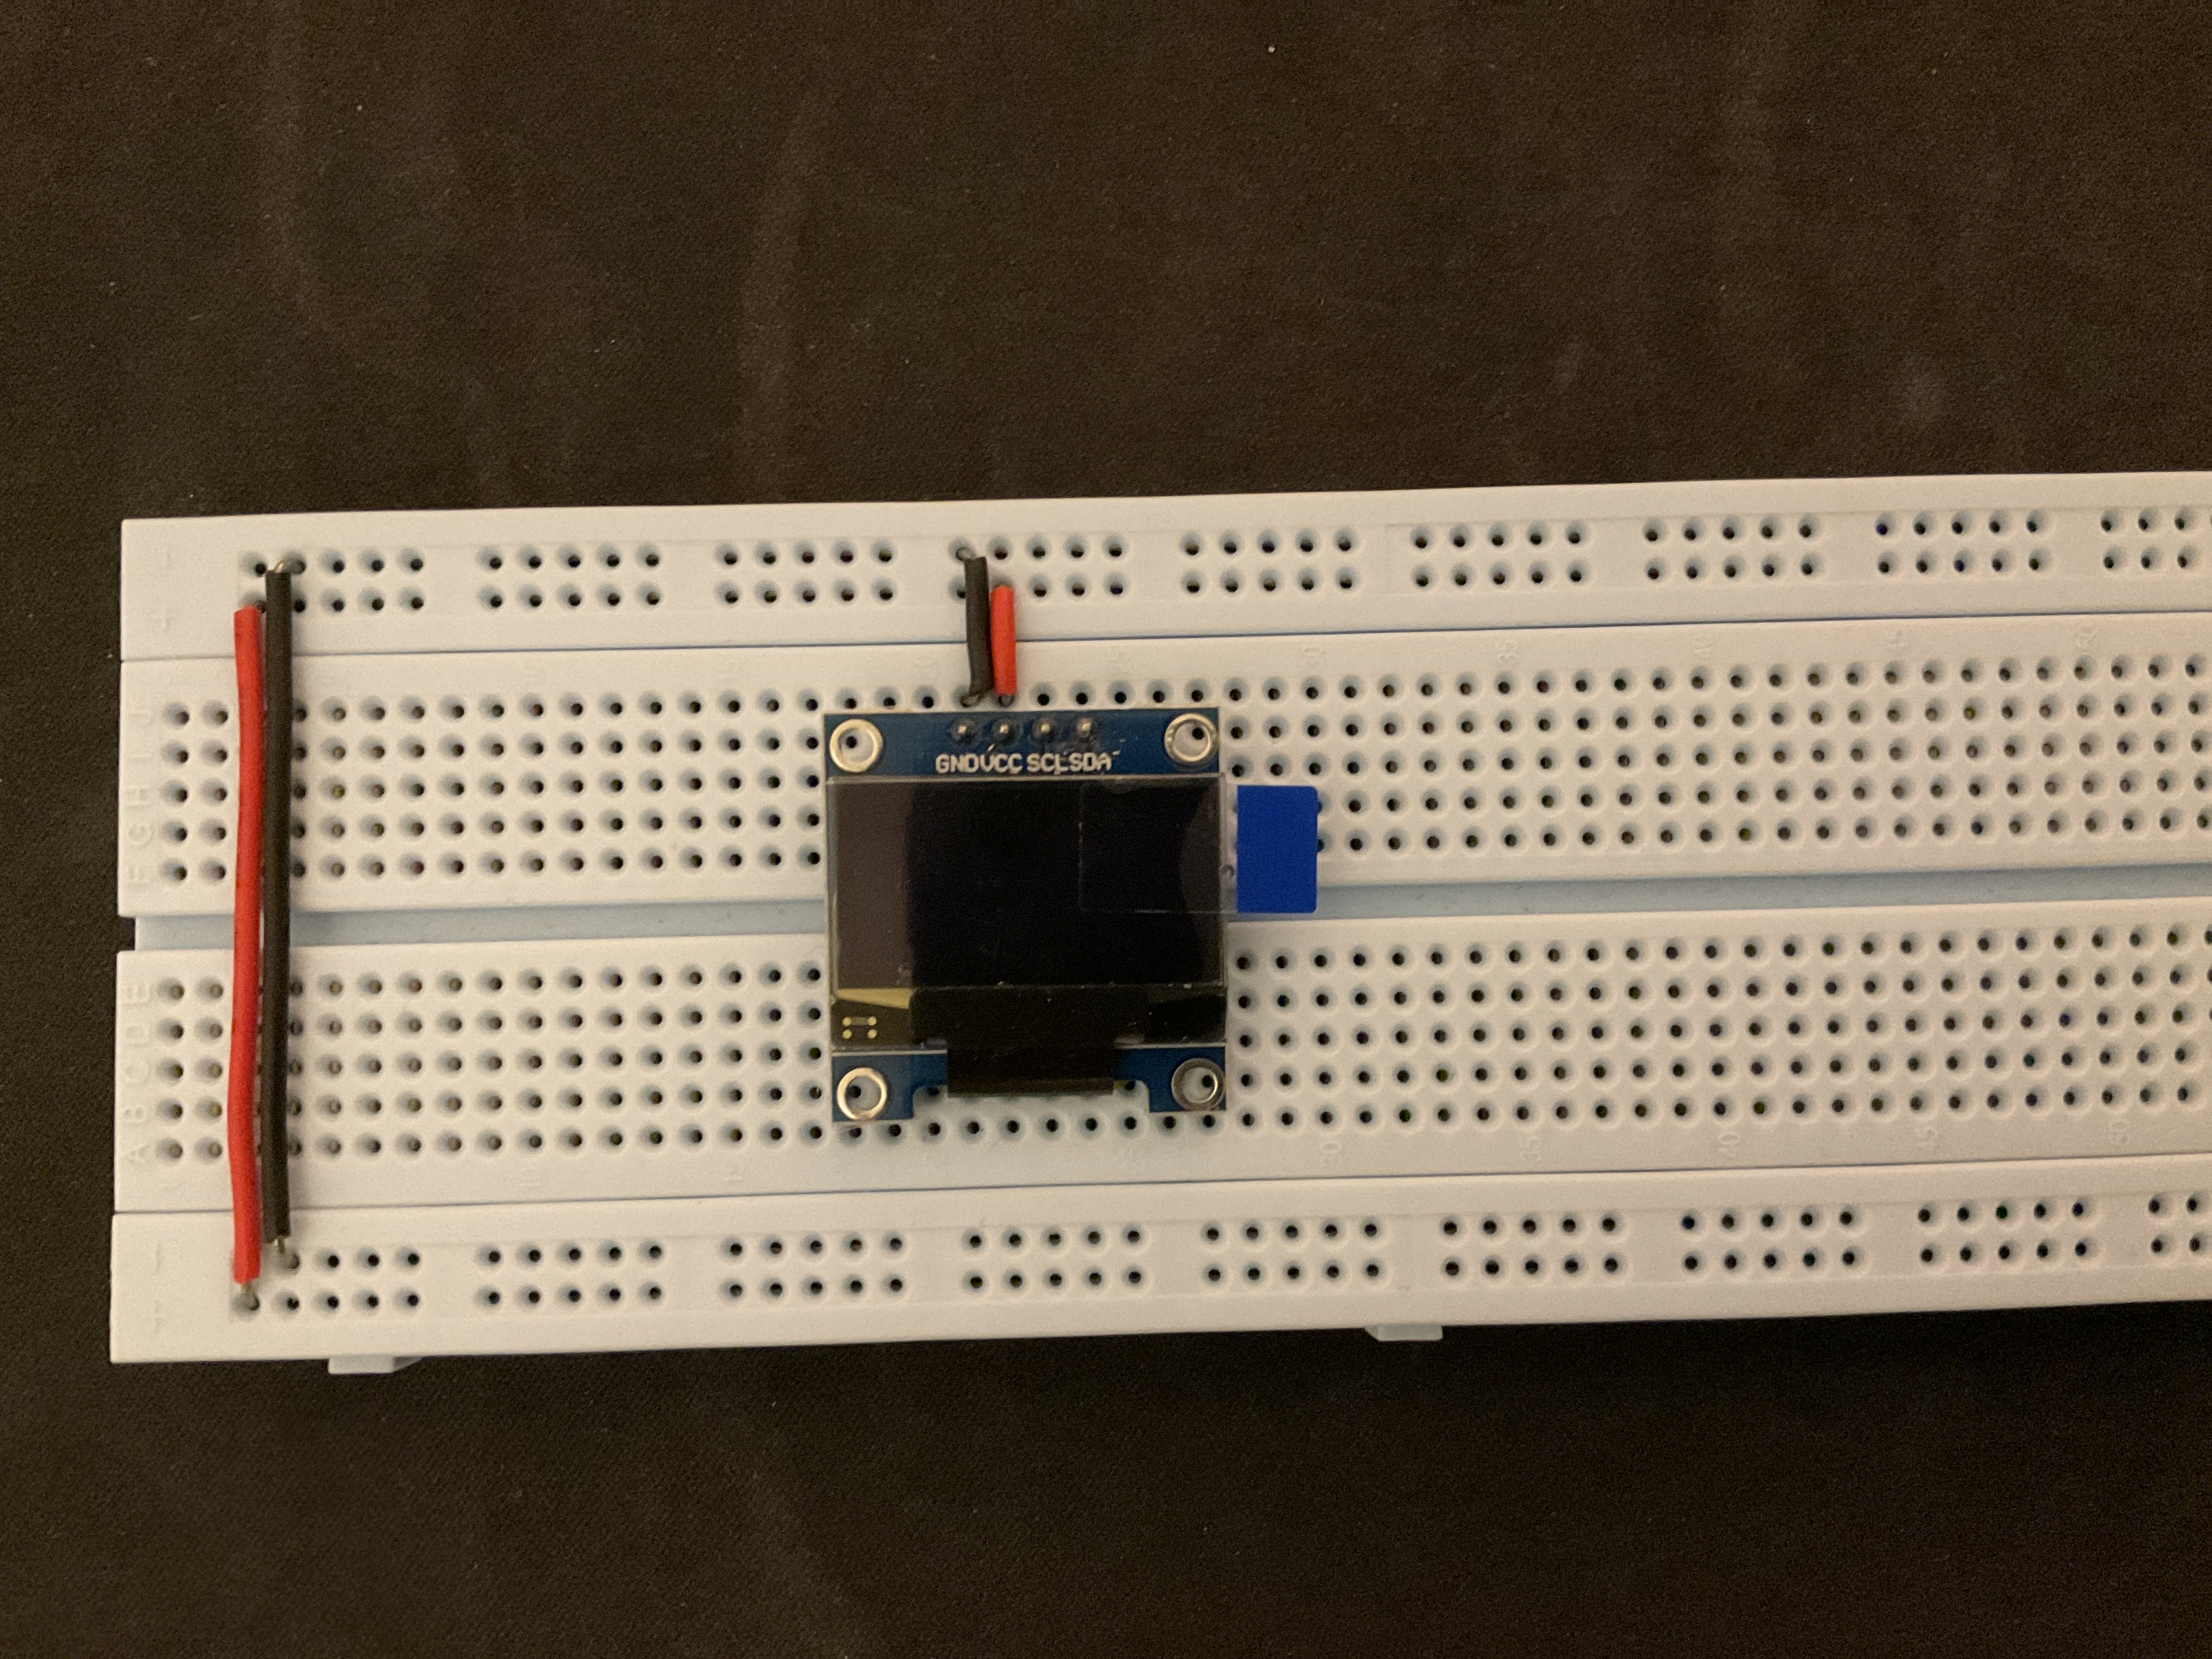
\includegraphics[width = .5\textwidth]{images/display.jpg}}
\end{center}
The SSD1306 has four pins that need to be tied down before operation can occur, they are labeled “GND”, “VCC”, “SCL”, and “SDA”. Ground and VCC were pretty easy so I tied them to their respective rails (VCC = 5V). Since I didn't know what SCL and SDA were I needed to find what they meant in the displays datasheet. After consulting the datasheet I found that SDA was the DATA Input, and SCL was the clock input. After connecting the Data input pin and the clock input pin to the proper analog pins on the arduino I downloaded the recommended libraries by the manufacturer, Adafruit, which are the Adafruit GFX library and the SSD1306 library. 

From there I decided to test to make sure that the display is properly functioning, so I loaded up one of the example codes that come with the arduino IDE which can be found by going to Files>Examples, and running that code to see if the intended output is produced. After doing this I got this output on the display:
\begin{center}
    \boxed{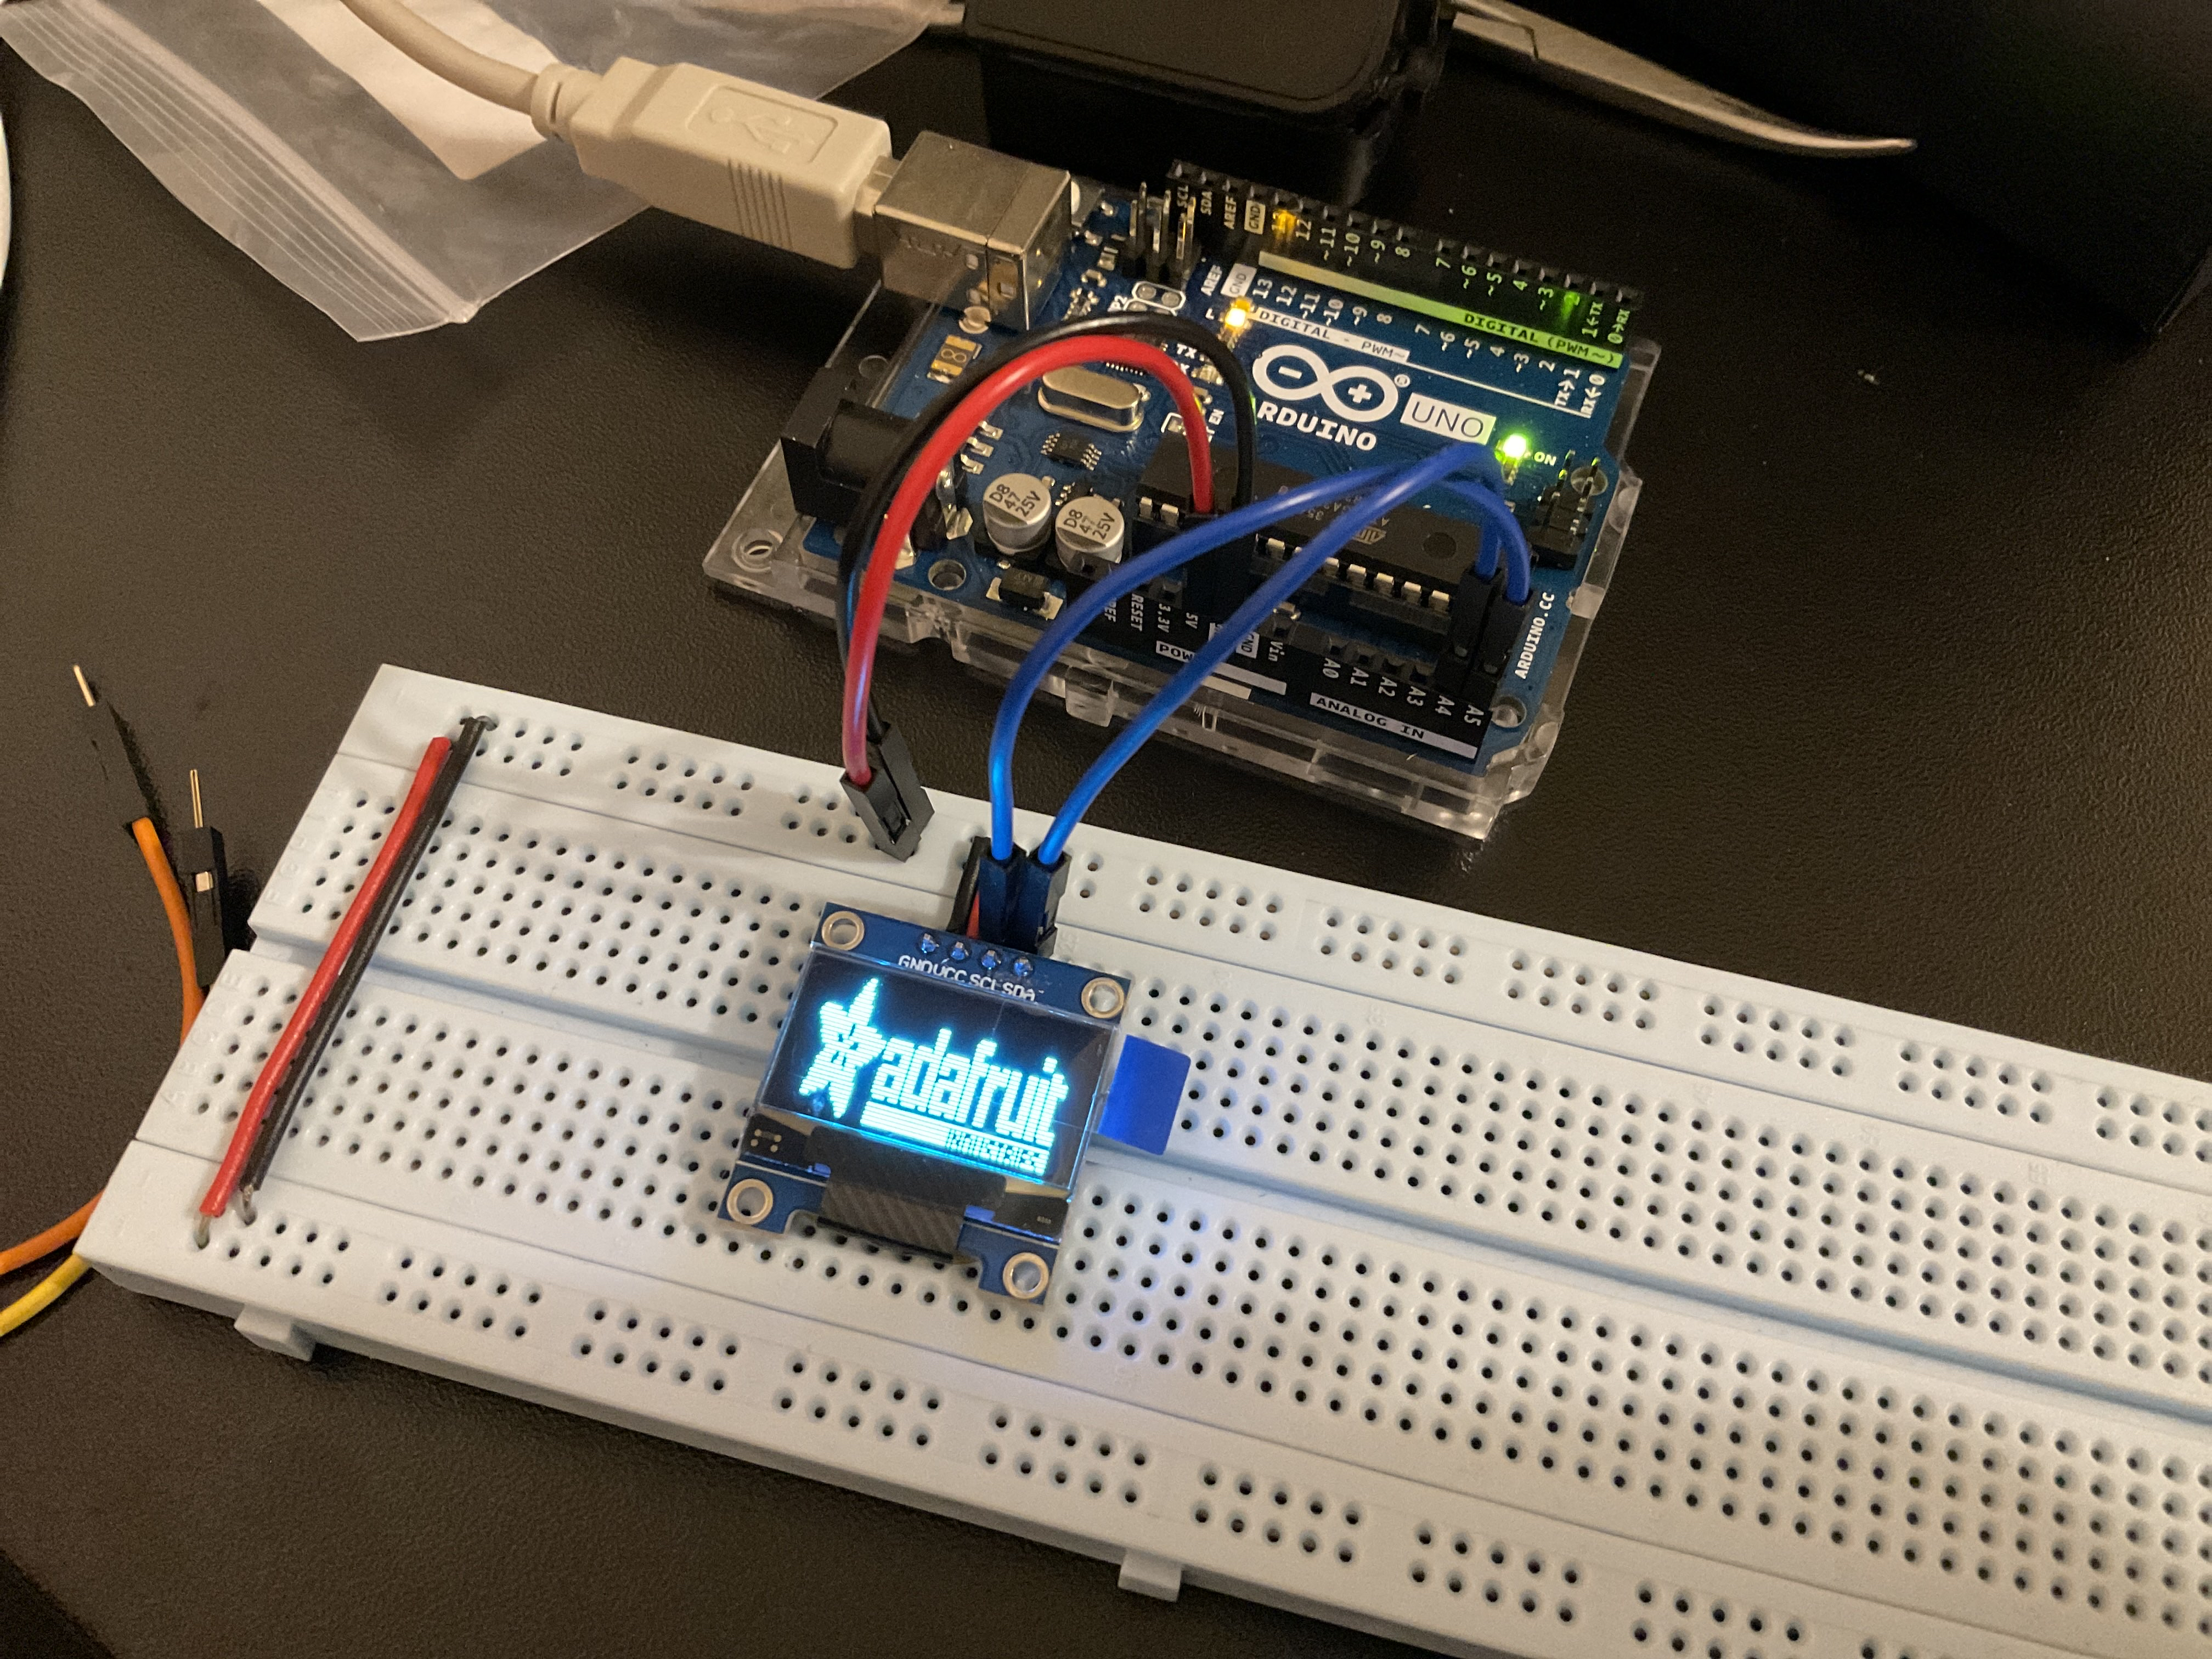
\includegraphics[width = .4\textwidth]{images/display_test.jpg}}
\end{center}
Now that I have a clear indication that my board is working correctly, I took some time to familiarize myself with some of the functions that are provided in the two libraries I downloaded. After looking through the documentation these were the commands that I thought to be the most important to know of the ones that I had looked at.
\begin{itemize}
    \item display.clearDisplay() –  turn all pixels off
    \item display.drawPixel(x,y, color) – plot a pixel in the x,y coordinates
    \item display.setCursor(x,y) – set the coordinates to start writing text
    \item display.print(“message”) – print the characters at location x,y
    \item display.display() – call this method for the changes to make effect
\end{itemize}
Using these functions I had found and taking guidance from the example code that came with the arduino IDE, I managed to create a simple proof of concept for the format of how the information that comes from the sensor will be processed and displayed as can be seen in the image below.
\begin{center}
    \boxed{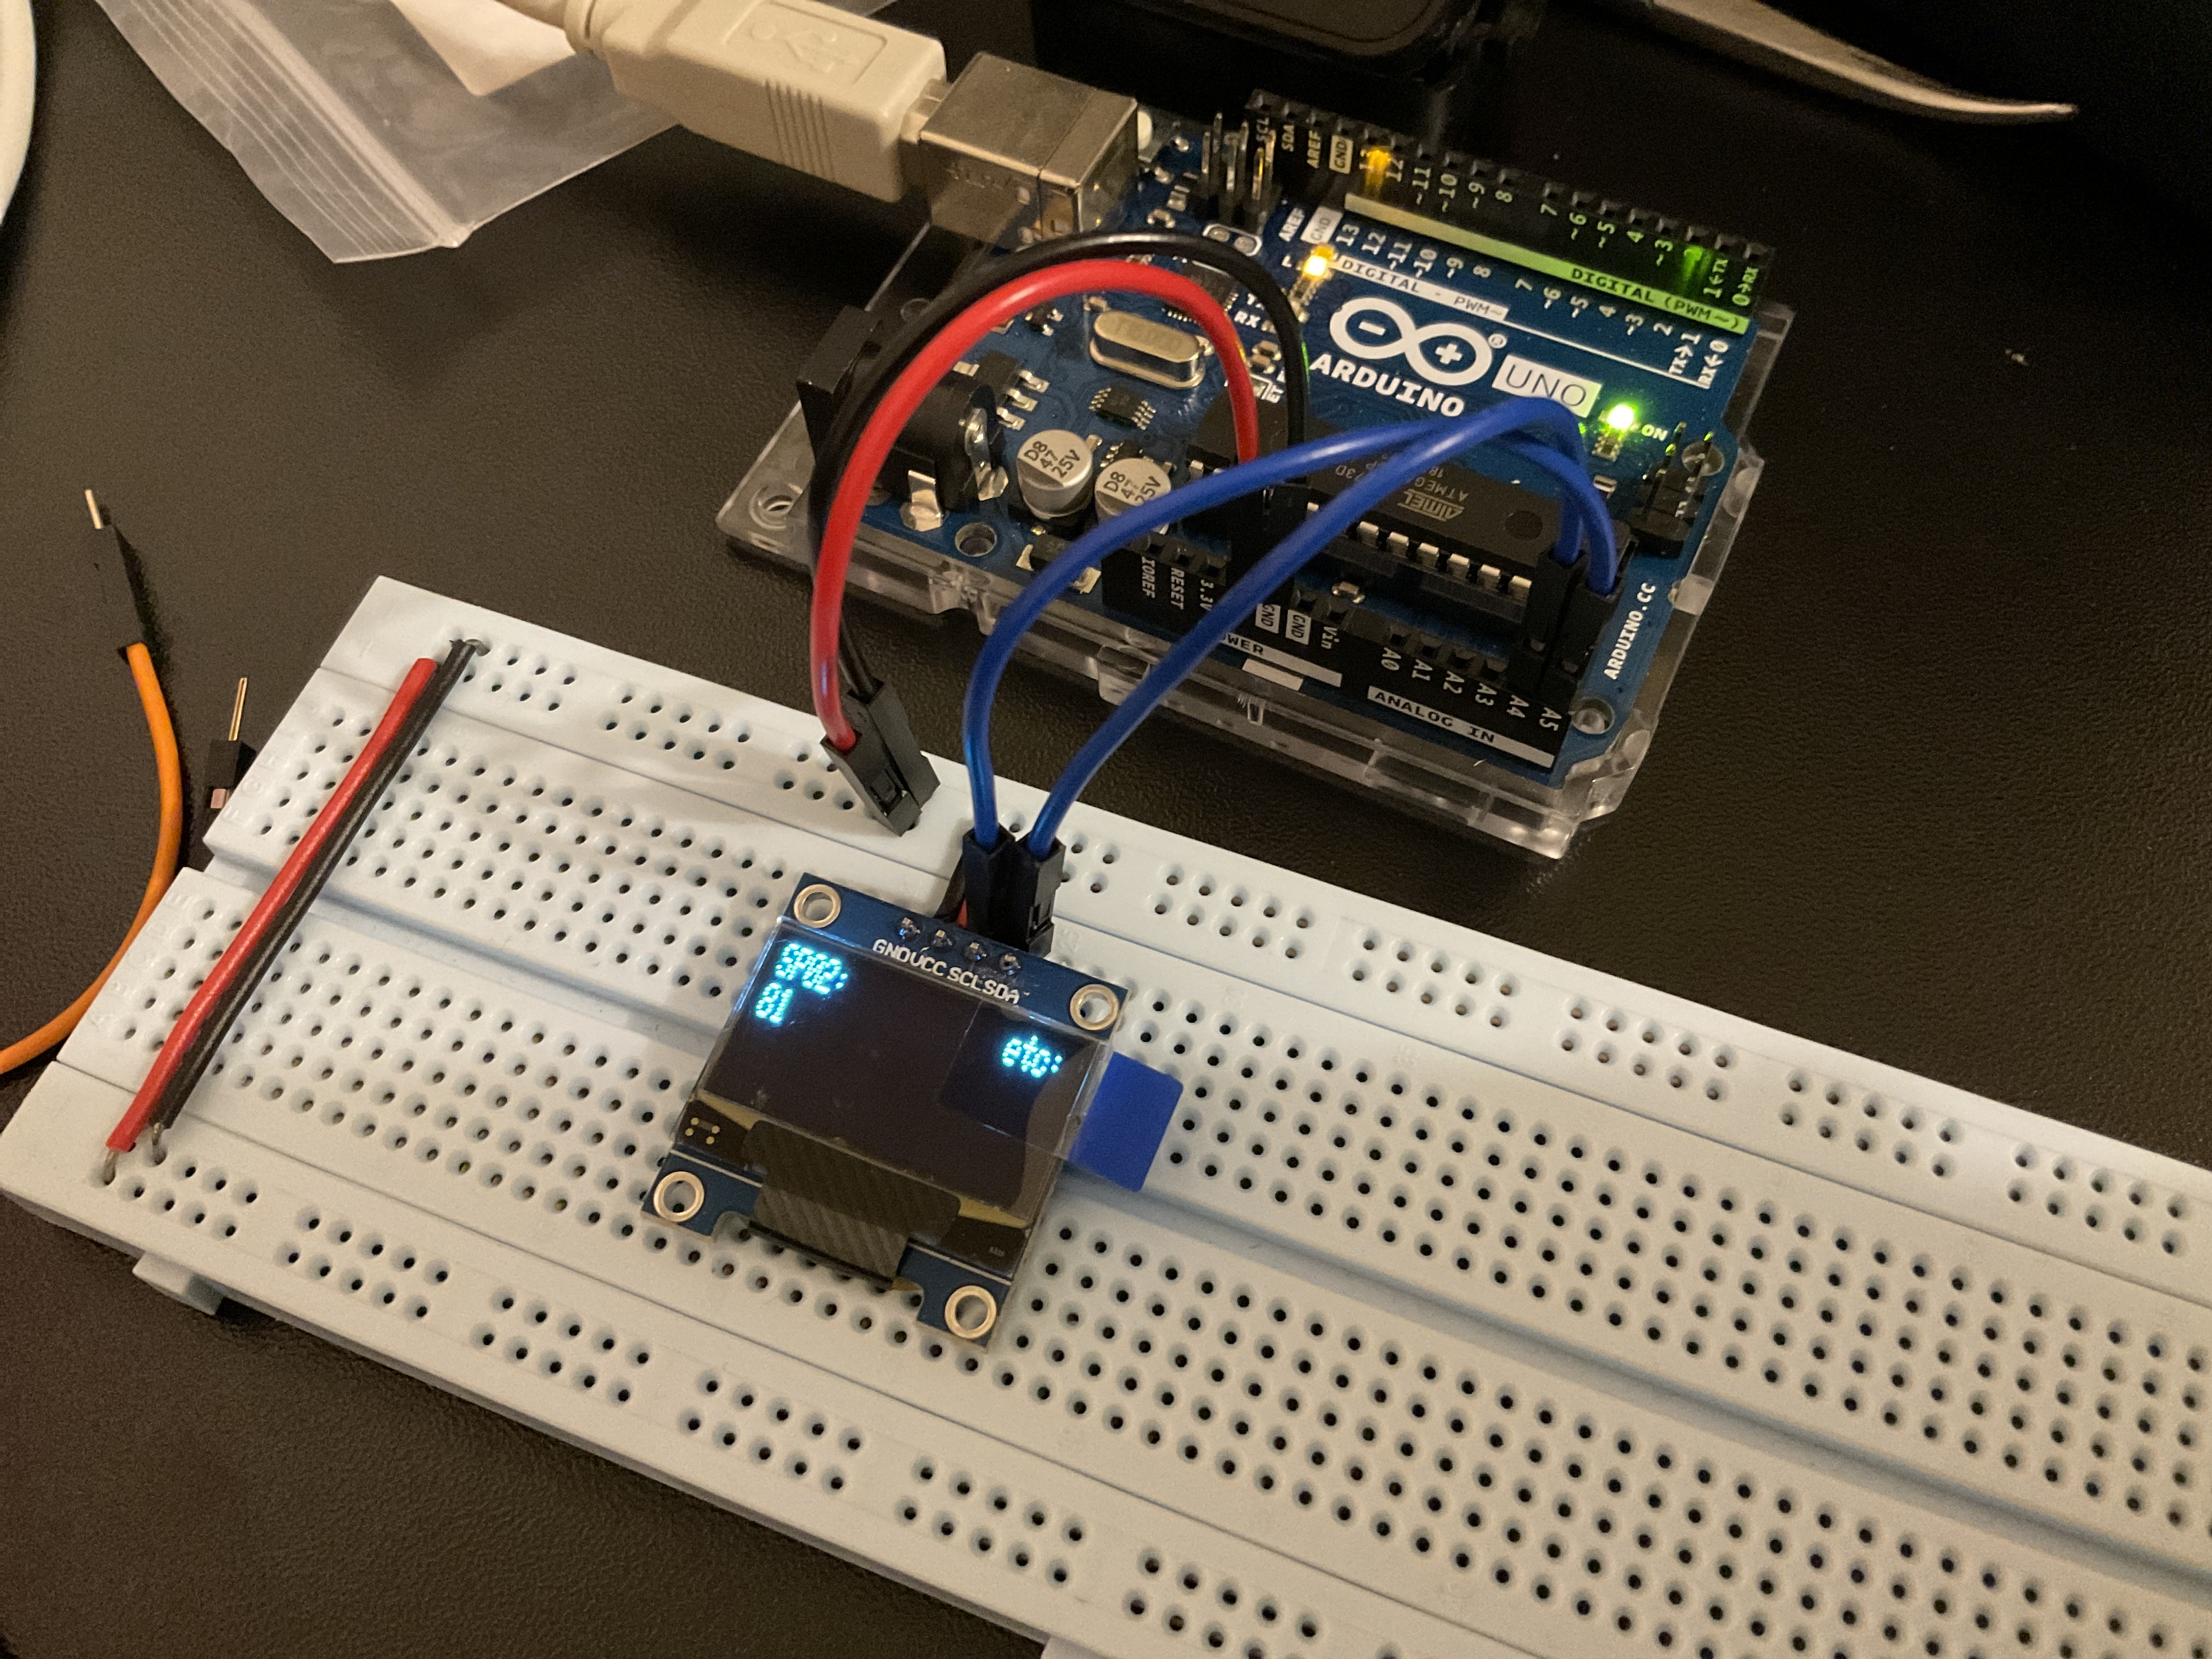
\includegraphics[width = .55\textwidth]{images/display_example.jpg}}
\end{center}
The number being displayed under the SPO2 label is just a simple loop going through a range of values that may or may not be those similar to the ones that will be displayed. Using these simple commands listed above it is possible to further expand this to a clean informative panel showing all required information. All that needs to be changed to move text or metrics is the cursor value in the (x,y) tuple format, (0,0) being the top left, and (128, 32) being the bottom right. In addition to adding more information to the display something that will be considered is the ability to interact with a potentiometer or button which would switch which screen the display is on making the need for the data to be small less important since it will allow us to have multiple “screens”. The code I made for this simple program Is listed below.
\begin{lstlisting}[language=Arduino, caption=Display Code]
#include <Wire.h>
#include <Adafruit_GFX.h>
#include <Adafruit_SSD1306.h> 

#define SCREEN_WIDTH 128 // OLED display width
#define SCREEN_HEIGHT 32 // OLED display height

Adafruit_SSD1306 display(SCREEN_WIDTH, SCREEN_HEIGHT, &Wire, -1);

void setup() {
  Serial.begin(9600);
  delay(2000);
  display.setTextSize(1);
  display.setTextColor(WHITE);
}

void loop() {
  for(int i = 0; i <= 100;i++){
    delay(100);
    display.clearDisplay();
    display.setCursor(0, 0);
    display.println("SP02:");
    display.setCursor(100, 0);
    display.println("etc:"); 
    display.setCursor(0, 9);
    display.println(i);
    display.display();
  }
}

\end{lstlisting}
All that needs to be changed in this code to display the correct information instead of a set of dummy values is that the “i” variable being used should be replaced with the variable holding the current value for whatever needs to be displayed in the certain place.
\newpage
Now that I had a grasp on how the display will be implemented, I decided to work on the data acquisition so that I could start to display real data on to the board instead of a simple FOR loop. For that I needed to start working with the arduino ADC, the approach I decided to take to doing this was to use the AD2 wave generator to create a wave, and then use the arduino ADC to take that analog wave and convert it back to digital, and once that is figured out I can plug that digital information into the SSD1306 display to test it with real data.
The first step I took in doing this was to create the circuit, it would just be the AD2’s wave gen funneled through the correct pins on the arduino as can be seen in the image below:
\begin{center}
    \boxed{\includegraphics[width = .95\textwidth]{images/adc_test.jpg}}
\end{center}

In the image, the wavegen is being run through a resistor to control current to where I want it to be, and directly after the resistor the node is connected to the A0 node of the arduino. Using to my surprise a very low amount of code I got the analog input and the arduino used its ADC to convert into digital the code is below

\begin{lstlisting}[language=Arduino, caption=ADC Test Code]
void setup() {
  Serial.begin(9600);
}

void loop() {
  Serial.println(analogRead(A0));
  Serial.print(" ");
}
\end{lstlisting}
\newpage
From there I used the IDE’s serial plotter to obtain a graph of what  the digital values look like. 
\begin{center}
    \boxed{\includegraphics[width = \textwidth]{images/adc_input.png}}
\end{center}
This is the image of what the AD2 oscilloscope is picking up.
\begin{center}
    \boxed{\includegraphics[width = \textwidth]{images/adc_output.png}}
\end{center}
And this is an image of the serial plotter output after the signal has been converted from analog to digital. It's not perfect, but it's a good starting point to further test and perfect to the point I want it to be at. Now I have a good foundation to be able to complete all the code for the display, ADC and Comparator blocks before milestone three.
\newpage
\section{Session 4 (Filter Redesign \& Peak/Valley Detection) [3 hours 26 minutes]}
I first decided to completely redo the filter stage and simulate, build, and test it

first I figured out what the most important aspect to filter out was and determined it was to ensure that any high frequencies were filtered out. This was to protect against effects from the systems power supply. For this a low-pass filter must be implemented. 

I decided to go with a second order filter so that we could be sure any noise is gone and also get some gain. I decided on an $A_v$ gain of 1.5, and a cutoff frequency of $f_b = 3Hz$ which would get rid of unwanted parts of the AC signal.

Based on those values I can calculate the resistor values like so:
\begin{align}
    A_v &= 1.5 \\
    &= 1 + \frac{R_f}{R_i}\\
    Let\text{ }&R_f = 47k\Omega\\
    R_i &= \frac{R_f}{A_v-1}\\
    &= \frac{47k\Omega}{1.5-1}\\
    &= 94k\Omega
\end{align}
\begin{center}
    So, $\boxed{R_f = 47k\Omega}$ and $\boxed{R_i \cong 100k\Omega}$
\end{center}
\begin{align}
    f_b &= 3Hz \\
    &= \frac{1}{2\pi RC}\\
    Let\text{ }&C = 1\mu F\\
    R &= \frac{1}{2\pi f_bC}\\
    &= \frac{1}{2\pi \cdot3Hz \cdot 1\mu F}\\
    &= 53051.648\Omega
\end{align}
\begin{center}
    So, $\boxed{C = 1\mu F}$ and $\boxed{R\cong 56k\Omega}$
\end{center}
Now we can build the circuit in LTSpice:
\begin{center}
    \boxed{\includegraphics[width = .8\textwidth]{images/ltfilter.png}}
\end{center}
\textbf{All values were rounded to values available in the kit} so the simulation should be a good representation of the reality.
\newpage
Now by using LTSpice's analysis we get the bode plot of the circuit.
\begin{center}
    \boxed{\includegraphics[width = .95\textwidth]{images/ltbode.png}}
\end{center}
As we can see the filter is serving its purpose and properly filtering out unwanted frequencies. Now that we know that the filter will serve our purpose we can build the circuit in real life and analyze it there.
\begin{center}
    \boxed{\includegraphics[width = .5\textwidth]{images/realfilter.jpg}}
\end{center}
Now that we have the real circuit constructed, using the oscilloscope and the wave form we can get the bode plot for the filter circuit.

From the bode plot we can see that the circuit is certainly filtering out the higher frequencies, \textbf{the range of the bode plot is a bit smaller since the data cannot be acquired nearly as quickly} as with the simulation as the trials actually need to occur at real time so for lower frequencies the trials can take upwards of an hour.
\begin{center}
    \boxed{\includegraphics[width = .9\textwidth]{images/realbode.png}}
\end{center}
Now we have a working filter with an input and output in an easily accessible place.

For peak valley detection, we need a differentiation circuit, so that when the derivative of the circuit is zero we can know that its a peak or valley

The reason why this is important, is because some versions of the heart rate formula need data at the peak or valley of the input signal, by having a differentiation circuit we can detect when the derivative of the input signal is zero and at that moment, sample the signal to be used in the formula.

The most basic form of an op-amp differentiator circuit would look something like this:
\begin{center}
    \ctikzset{
    bipoles/length=1.15cm,
    transistors/scale=1.4,
    grounds/scale=1.4, 
    tripoles/mos style/arrows
    }
    \begin{circuitikz}[scale=0.7, transform shape]
        \draw node[op amp](a){};
        \draw (a.+) to [short] ($(a.+)+(-.25,0)$) node[ground]{};
        \draw (a.-) to [short,-*] ($(a.-)+(-.25,0)$)
        to [C,l=$C$] ($(a.-)+(-2.25,0)$);
        \draw ($(a.-)+(-.25,0)$) to [short] ($(a.-)+(-.25,.75)$)
        to [R,l=$R$] ($(a.east)+(.25,1.17)$)
        to [short,-*] ($(a.east)+(.25,0)$)
        to [short] (a.east);
        \draw ($(a.east)+(.25,0)$) to [short] ($(a.east)+(1,0)$);
    \end{circuitikz}
\end{center}
The problem with this design is that it is rather unstable and can break at higher frequencies, in  addition the equation that describes this circuit is:
\begin{equation}
    V_{out} = -RC\frac{dV_{in}}{dt}
\end{equation}
As we can see it has a negative gain, so to improve this circuit we need to add some components to the differentiator and in addition have an inverting opamp with an $A_v$ gain of 1. After taking this into consideration, we get the following circuit:
\begin{center}
    \ctikzset{
    bipoles/length=1.15cm,
    transistors/scale=1.4,
    grounds/scale=1.4, 
    tripoles/mos style/arrows
    }
    \begin{circuitikz}[scale=0.7, transform shape]
        \draw node[op amp](a){};
        \draw (a.+) to [short] ($(a.+)+(-.25,0)$) node[ground]{};
        \draw (a.-) to [short,-*] ($(a.-)+(-.25,0)$)
        to [C,l=$C_1$]($(a.-)+(-2.25,0)$)
        to [R,l=$R_1$]($(a.-)+(-4.25,0)$);
        \draw ($(a.-)+(-.25,0)$) to [short] ($(a.-)+(-.25,.75)$)
        to [R,l=$R_2$] ($(a.east)+(.25,1.17)$)
        to [short,-*] ($(a.east)+(.25,0)$)
        to [short] (a.east);
        \draw ($(a.-)+(-.25,.75)$) to [short] ($(a.-)+(-.25,2)$)
        to [C,l=$C_2$]($(a.east)+(.25,2.42)$) 
        to [short]($(a.east)+(.25,1.17)$);
        \draw ($(a.east)+(.25,0)$) to [short] ($(a.east)+(1,0)$);
        \draw (5.2,-.4025)node[op amp](b){};
        \draw (b.+) to [short] ($(b.+)+(-.25,0)$) node[ground]{};
        \draw (b.-) to [short,-*] ($(b.-)+(-.25,0)$)
        to [R,l=$R_i$] ($(b.-)+(-2.25,0)$);
        \draw ($(b.-)+(-.25,0)$) to [short] ($(b.-)+(-.25,.75)$)
        to [R,l=$R_f$] ($(b.east)+(.25,1.17)$)
        to [short,-*] ($(b.east)+(.25,0)$)
        to [short] (b.east);
        \draw ($(b.east)+(.25,0)$) to [short] ($(b.east)+(1,0)$);
    \end{circuitikz}
\end{center}
Now we need to calculate the values for the resistors and capacitors in the circuit:
\begin{center}
    We want an $A_v$ gain of 1 so:
\end{center}
\begin{equation}
    R_i = R_f\text{ and }R_2 = \frac{1}{C_1}
\end{equation}
\begin{center}
    Let $C_1 = 10\mu F$:
\end{center}
\begin{equation}
    R_2 = \frac{1}{10\mu F} = 100k\Omega
\end{equation}
\begin{center}
    So, $\boxed{C_1 = 10\mu F}$ and $\boxed{R_2 = 100k\Omega}$
\end{center}
\begin{center}
    We also have that:
\end{center}
\begin{equation}
    R_1 = \frac{1}{2}\sqrt{R_2/C_1f_T}\text{ and }C_2 \cong C_1R_1/R_2
\end{equation}
Now to calculate the rest of the values we need the transit frequency $(f_T)$ of the op-amp, our op-amp (LF356N) the data sheet is:

\url{https://www.ti.com/lit/ds/symlink/lf356.pdf?ts=1617382462054&ref_url=https%253A%252F%252Fwww.ti.com%252Fproduct%252FLF356}

\begin{center}
    \boxed{\includegraphics[width = .85\textwidth]{images/gain_bandwidth.png}}
\end{center}
From the datasheet we can see that  $f_T$ is $5MHz$.

Now with all the information we need we can calculate the rest of the values in the circuit
\begin{align}
    R_1 &= \frac{1}{2}\sqrt{\frac{R_2}{C_1f_T}} \\
    &= \frac{1}{2}\sqrt{\frac{100k\Omega}{10\mu F\cdot 5MHz}}\\
    &= \frac{\sqrt{2}}{2}\Omega
\end{align}
\begin{equation}
    C_2 = 7.07\cdot 10^{-11}
\end{equation}
\begin{center}
    So, $\boxed{C_2 = 7.07\cdot 10^{-11}}$ and $\boxed{R_1 = \frac{\sqrt{2}}{2}\Omega}$
\end{center}
The values that have been calculated here are small enough to be negligible, which means in this situation the inefficient op-amp is virtually as good as the efficient one.

Finally, we can pick two arbitrary values for $R_i$ and $R_f$ as long as they are the same, so
\begin{center}
    So, $\boxed{R_i = 50k\Omega}$ and $\boxed{R_f = 50k\Omega}$
\end{center}
Now we can make the circuit in LTSpice.
\begin{center}
    \boxed{\includegraphics[width = .75\textwidth]{images/ltdifferentiator.png}}
\end{center}
With this new circuit we can run a simulation to see if the differentiation effect is occurring.
\begin{center}
    \boxed{\includegraphics[width = \textwidth]{images/ltdifferentiation_plot.png}}
\end{center}
As can be seen the original sin function was differentiated into a cosine function.
\newpage
\section{Session 5 (Final Filter Design) [1 hours 35 minutes]}
After receiving critique about having gain on my previous filter redesign I decided to once again redo the filter stage, this time by using a two stage Bessel filter which will be sure to get rid of any noise and 60Hz hum very quickly. Therefore I had an $A_v$ gain of 0, and a cutoff frequency of $f_b = 3Hz$ which would get rid of unwanted parts of the AC signal.

This time I decided to use the Filter Design Tool by Analog:

\url{https://tools.analog.com/en/filterwizard/}
\begin{align}
    f_b &= 3Hz \\
    &= \frac{1}{2\pi RC}\\
    Let\text{ }&C = 1\mu F\\
    R &= \frac{1}{2\pi f_bC}\\
    &= \frac{1}{2\pi \cdot3Hz \cdot 1\mu F}\\
    &= 53051.648\Omega
\end{align}
Using their tool I could input the desired passband and stopband values and I got $R = 53k\Omega$ and $C = 1\mu F$ for my component values. Now I can build the circuit in LTSpice after rounding component values to those available in the kit, and test it there.
\begin{center}
    \boxed{\includegraphics[width = .9\textwidth]{images/ltfilter_final.png}}
\end{center}
Now with a LTSpice diagram I can test this with a simple frequency sweep and get the bode plot for the circuit
\begin{center}
    \boxed{\includegraphics[width = \textwidth]{images/ltbode_final.png}}
\end{center}
Now I can build the circuit in real life to get a bode plot simulation from that.
\begin{center}
    \boxed{\includegraphics[width = .75\textwidth]{images/double_filter_bode.png}}
\end{center}
As it is the ~1Hz are being slightly attenuated, so in the future I may change this so that the main heart rate component of the signal can get past without getting eaten. So instead of a $f_b$ of 3Hz, I may change it to around 10Hz.
\begin{center}
    \boxed{\includegraphics[width = .475\textwidth]{images/red_output.png}}
    \boxed{\includegraphics[width = .475\textwidth]{images/filtered_ppg.png}}
\end{center}
Now we have a filtered PPG signal which is much easier to read and will give us more information than before, for example with the differentiating circuit there will not be issues as there are no longer high frequency components that would constantly be hitting zero.
\newpage
\section{Session 6 (Multiplexer) [3 hours 2 minutes]}
First thing to do this week is to figure out the multiplexer. To do this I plugged the mux into the board, and read the model number using that to find the data sheet for the mux.
\begin{center}
    \boxed{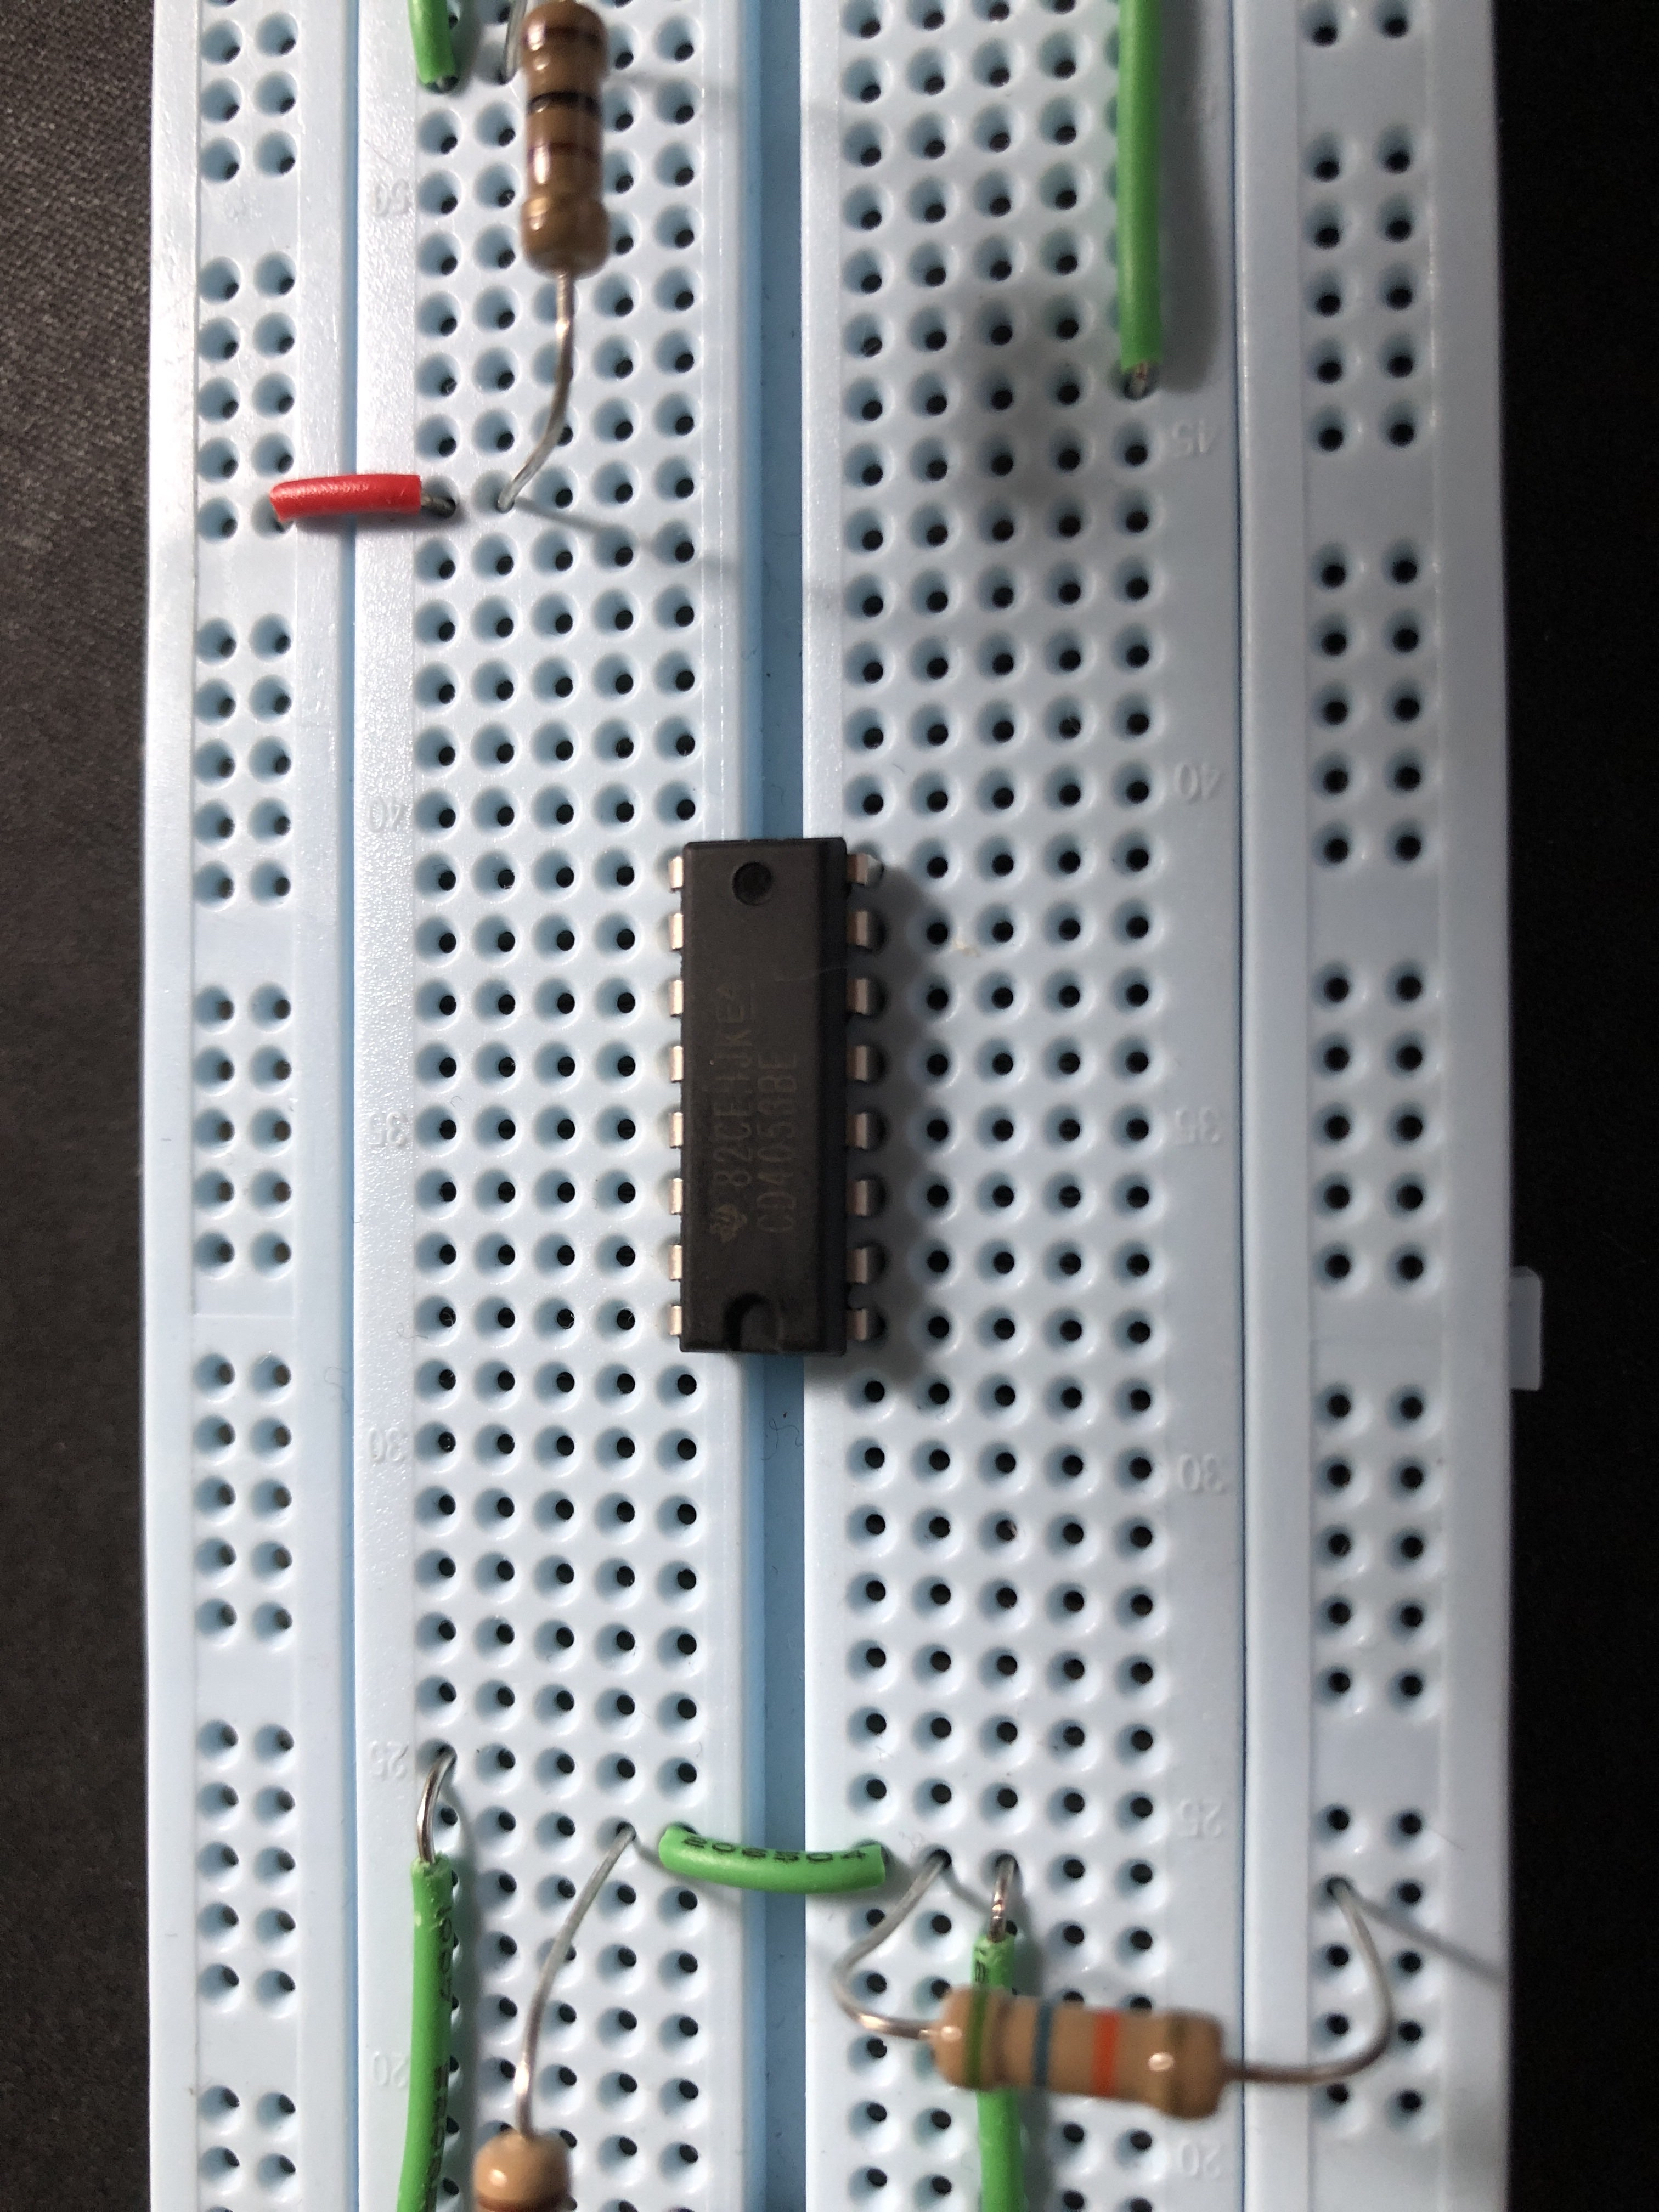
\includegraphics[width = .75\textwidth,height = .5\textwidth]{images/mux.jpg}}
\end{center}
From this we can see that the model number is \textbf{CD4053BE}. From this the datasheet can be found to be here at the following link:

\url{https://www.ti.com/general/docs/suppproductinfo.tsp?distId=10&gotoUrl=http%3A%2F%2Fwww.ti.com%2Flit%2Fgpn%2Fcd4051b}

Now we can get the pin-out from the data sheet to better understand the multiplexer:
\begin{center}
    \boxed{\includegraphics[width = .475\textwidth]{images/pinout.png}}
\end{center}
Now I can start by making the easiest connections first, $V_{DD}$ and $V_{SS}$(Ground) but first I need to find out how many volts the $V_{DD}$ on this chip is rated for. 
\begin{center}
    \boxed{\includegraphics[width = .65\textwidth]{images/maxratings.png}}
\end{center}
Now that I know I can safely tie $V_{DD}$ to 5V without damage I can give the mux $V_{SS}$ and $V_{DD}.$

The next step before I can test the operation of the mux is to use the datasheet to figure out the purpose of all of the remaining pins and to decide wether or not I need to use them.
\begin{itemize}
    \item \textbf{PIN 6:INH}
    
    INH stands for inhibit, this pin if given a logic level of one will stop the operation of the multiplexer completely, could be useful for a bonus feature for pausing or such, but for now I will tie it to ground since we want the multiplexer actually operating.
    
    Input: GND
    \item \textbf{PIN 7:$V_{EE}$}
    
    This input is the negative voltage source, according to the data sheet it seems like this is a needed input for operation of the multiplexer so I will be connecting it properly.
    
    Input: -5V
    \item \textbf{PIN OTHER:[ax, ay, bx, by, cx, cy]}
    
    These pins are the input/output pins for the multiplexers and it does work in both directions, so if needed It can decode.
    
    Input: Desired Signal
    \item \textbf{PIN 11-9:[A, B, C]}
    
    These three channels are the select bits for the multiplexer, the inputs needed to pass the correct output can be seen in the truth table below.
    
    Input: Sel Bits
\end{itemize}
\begin{center}
    \boxed{\includegraphics[width = .55\textwidth]{images/truthtable.png}}
\end{center}
After a bit of research I realized that instead of this being a 3x8 multiplexer, it is 3 1x2 multiplexers, which makes things pretty simple as I don't need to use most of those inputs to the multiplexer anyway.

After figuring out the purposed of the pins, this is the mini-circuit I ended up with.
\begin{center}
    \boxed{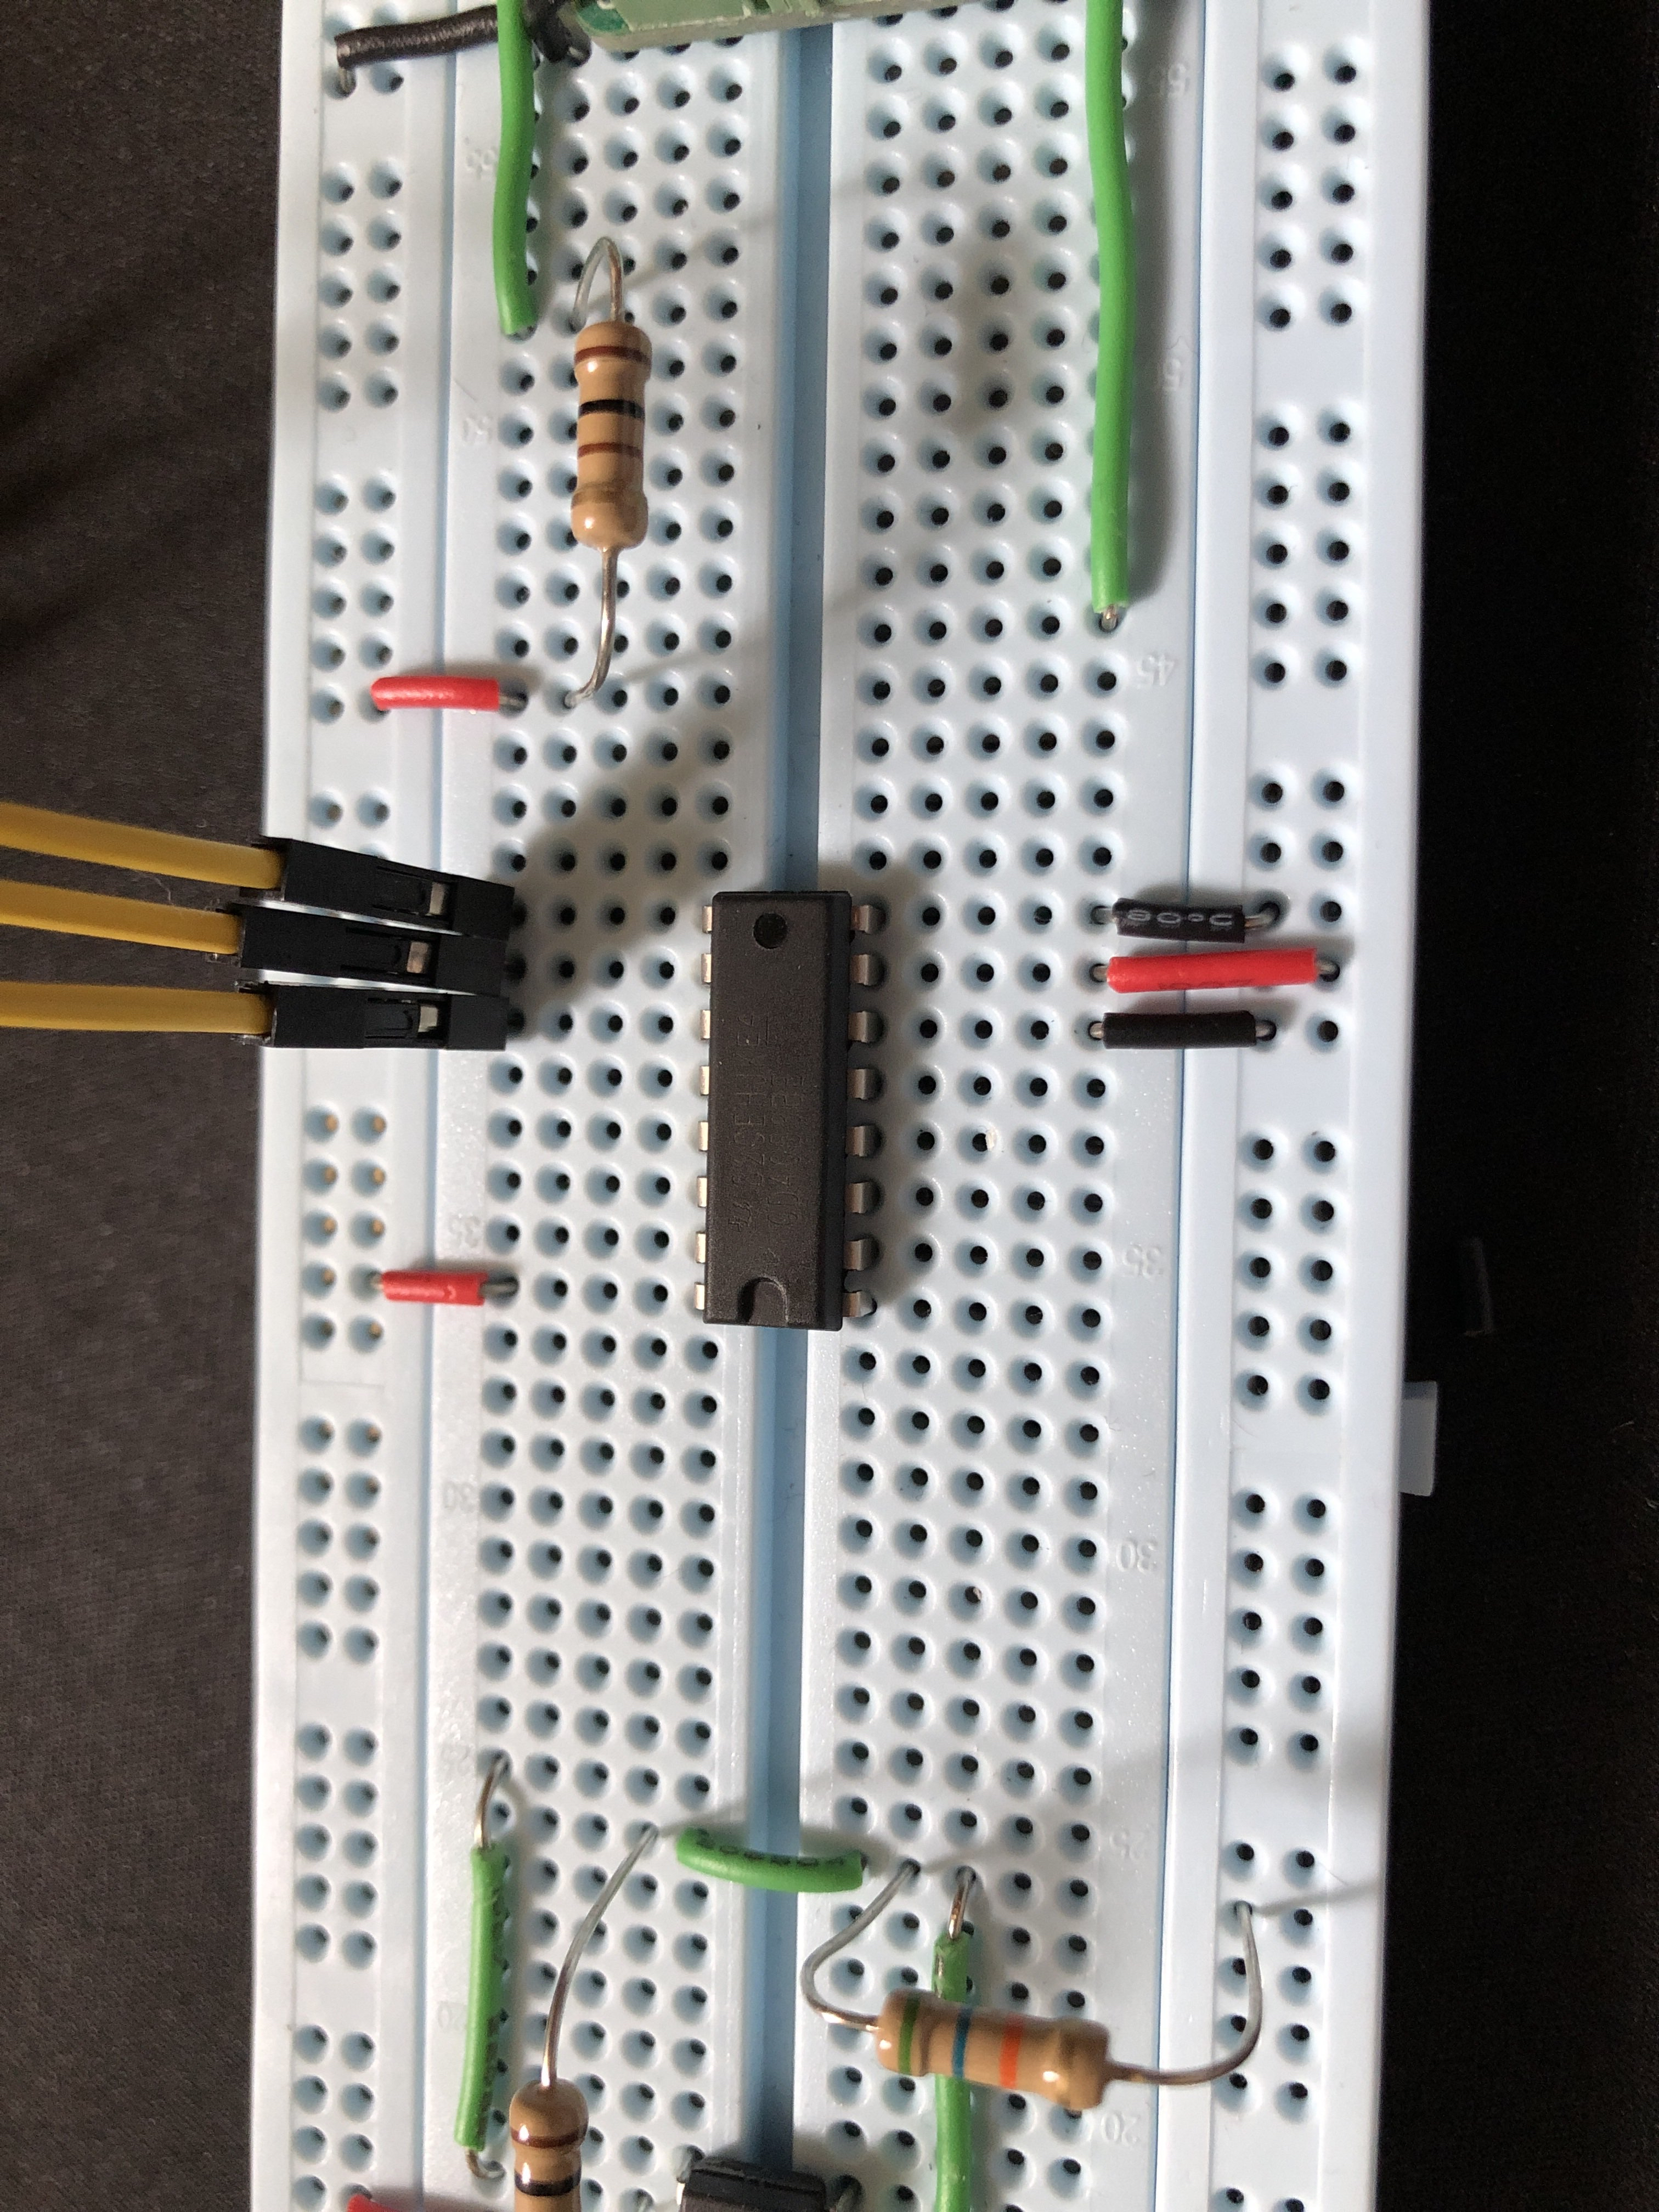
\includegraphics[width = .65\textwidth,height = .45\textwidth]{images/mux2.jpg}}
\end{center}
Now I can write some simple test code in the arduino to test out the multiplexer A.
\begin{lstlisting}[language=Arduino, caption=Multiplexer Test Code]
void setup() {
  pinMode(13, OUTPUT); // primes pin 13 for digital writing
}

void loop() {
  digitalWrite(13, HIGH); // sets the digital pin 13 on
  delay(500);            // waits for a half second
  digitalWrite(13, LOW);  // sets the digital pin 13 off
  delay(500);            // waits for a half second
}
\end{lstlisting}
Now this code will send the A select bit a high signal, then a low signal continuously which will switch the input and outputs of the multiplexer, now I need to provide the mux with proper inputs. I can do this using both channels of the wavegenerator on the AD2.
\begin{center}
    \boxed{\includegraphics[width = .85\textwidth]{images/wavegen.png}}
\end{center}
Now in theory when I turn on all components, on the oscilloscope I should see a signal that switches between noise and sin wave every half a second. If this doesn't happen I can debug and go from there.
\begin{center}
    \boxed{\includegraphics[width = .85\textwidth]{images/oscillisocpe_mux.png}}
\end{center}
Now that the multiplexer is setup when the time comes to select the proper signal input from the sensor it can be done.
\newpage
\section{Session 7 (Lots of Stuff) [14 hours 12 minutes]}
\subsection{Post-Filtering Amplification}
With the filtering done we need to amplify the signal even more to make it more visible and manipulable. I will be using a simple non-inverting op amp for this. Start with some simple calculations for the component values. 
\begin{center}
    \ctikzset{bipoles/length=1cm,transistors/scale=1.4,grounds/scale=1.4}
    \begin{circuitikz}[scale=1]
        \ctikzset{tripoles/mos style/arrows}
        \draw (0,0) to [vsourcesin,l=$v_i$](0,2)
        to [R,l=$R_{Si}$](1.5,2)
        to [C,l=$C_{C1}$](3,2)
        to [R,l_=$R_1$] (3,4)
        to [short,-*] (3.75,4)
        to [short, -o](3.75,4.5) node[anchor=south]{$V_{DD}$}
        (3.75,4) to [short,-] (4.5,4)
        to [R,l=$R_D$,-*] (4.5,2.75)
        to [short, -o](5.25,2.75)node[anchor=west]{$v_o$};
        \draw (3,2) to [short,*-] (3.51,2)(4.5,2) node[nmos]{};
        \draw (0,0) to [short, -*] (3,0) to [R,l_=$R_2$] (3,2) 
        (3,0) to [short, -*](4.5,0) node[ground]{} to [short] (4.5,1.22);
    \end{circuitikz}
\end{center}
There is alot of uncertainty with the transistor parameters for the transistors in our kit because they are not listed anywhere, but from experience and from ECE2214 labs I have learned that $K_n \cong 30\frac{mA}{V^2}$ and $V_{TN} \cong 1.1V$ so those are the values I will use for the transistor parameters. I want a gain so that I will be able to see the final signal but I also need to make sure I dont go under 0 volts or over 5 volts so that will be reflected in the calculations.
\begin{equation}
    5mA = 30\frac{mA}{V^2}(V_{DS}(sat))^2 \Rightarrow V_{DSt} = .408V
\end{equation}
\begin{equation}
    V_{DSQ} = \frac{V_{DD}+V_{DSt}}{2}= 2.7V
\end{equation}
\begin{center}
\end{center}
\begin{align}
    V_{DD} &=  I_{DQ}R_D + V_{DSQ}\\
    \Rightarrow 5V &=  2.5mA\cdot R_D + 2.7V\\
    \Rightarrow R_D &=  \boxed{920\Omega}
\end{align}
\begin{align}
    2.5mA &= 30\frac{mA}{V^2}(V_{GSQ}-1.1V)^2\\
     V_{GSQ} &= \pm\sqrt{\frac{2.5mA}{30\frac{mA}{V^2}}} + 1.1V\\
     V_{GSQ} &= 1.38867V
\end{align}
\begin{align}
    V_{GSQ} &= V_{DD}\left(\frac{R_2}{R_1+R_2}\right)\\
    \Rightarrow R_1\cdot V_{GSQ} &= V_{DD}(R_1||R_2)\\
    \Rightarrow R_1\cdot1.258V &= 5V\cdot100k\Omega\\
    \Rightarrow R_1 &= \boxed{360k\Omega}\\
    \Rightarrow R_2 &= \frac{V_{GSQ}R_1}{V_{DD}-V_{GSQ}}\\
    &= \boxed{138.453k\Omega}
\end{align}
\newpage
Here is the small signal equivalent for the MOSFET amplifier above.
\begin{center}
    \ctikzset{bipoles/length=1cm,transistors/scale=1.4,grounds/scale=1.4}
    \begin{circuitikz}[american currents,american voltages]
        \ctikzset{tripoles/mos style/arrows}
        \draw
        (-1.5,0) to [vsourcesin,l=$v_i$](-1.5,2)
        to [short](.5,2)
        (-1.5,0) to [short](0,0)
        (-.6,0) to [R,l_=$R_1$,*-*](-.6,2)
        (.4,0) to [R,l_=$R_2$,*-*](.4,2)
        to [short, -o](1.5,2)node[anchor=south]{G}
        to [open,v=$V_{GS}$](1.5,0)
        (0,0) to [short,-*](1.5,0)
        to [short](3,0)
        (3,0) to [short,-o](7,0)
        (3,0) node[anchor=north]{S} to [cisource,l_=$V_{GS} g_m$,invert,*-](3,2)
        to [short](5,2)
        to [short](6.5,2)
        to [short, -o](7,2)node[anchor=west]{$v_o$}
        (6,2) to [R,l=$r_o$,*-*](6,0)
        (5,2)node[anchor=south]{D} to [R, l=$R_D$,*-*](5,0);
    \end{circuitikz}
\end{center}
\begin{equation}
        A_v = -g_m(r_o||R_D) = -2\sqrt{30\frac{mA}{V^2}\cdot 2.5mA} \cdot 920\Omega = \boxed{-15.93486}
\end{equation}
\begin{center}
    So, $\boxed{R_1 = 360k\Omega}$, $\boxed{R_2 = 140k\Omega}$, and $\boxed{R_D = 920\Omega}$
\end{center}
Since this amplifier has a negative gain I also need an inverting op amp with a gain of 1 to normalize the signal after its amplified
\begin{equation}
    A_v = \frac{R_f}{R_i} \Rightarrow R_f = R_i
\end{equation}
\begin{center}
    So all I need to do to make the amplifier is pick two resistor values which are equal to each
    
    So, $\boxed{R_f = 100k\Omega}$ and $\boxed{R_i = 100k\Omega}$
\end{center}
\begin{center}
    \boxed{\includegraphics[width = .75\textwidth]{images/LTcommonsource.png}}
\end{center}
Now we can test it, but to see any meaningful information I need to graph the output in an external program such that I can give $V_{out}$ an offset off $V_{DSQ}$, I chose to do that in python. The code I used for this is below:
\begin{lstlisting}[language=Python, caption= Graphing Code]
import numpy as np
import matplotlib.pyplot as plt
from matplotlib.pyplot import figure
import pandas as pd

figure(figsize=(14, 6))

# import csv and convert to numpy array

real = pd.read_csv("C:\Users\ksbkt\OneDrive - Virginia Tech\Documents\Files\School\ECE2804\project\commonsource.csv", names=["time", "V_IN", "V_OUT"])

real.time *= 10**3
real.V_OUT *= 10**3
real.V_IN *= 10**3

# plot

plt.title("NMOS Amplifier: Physical")
plt.plot(real.time, real.V_IN, label="$V_{IN}$")
plt.plot(real.time, (real.V_OUT-4.95*10**3), label="$V_{OUT}$")
plt.xlabel("$Time(ms)$ ")
plt.ylabel("$Voltage(mV)$")
plt.legend()
plt.show()
\end{lstlisting}
\begin{center}
    \boxed{\includegraphics[width = .6\textwidth]{images/nmosampsim.png}}
\end{center}
So we clearly have a good amount of gain that will allow us to properly play around with ours signal, now I can build the circuit in real life and connect it up to the output of the filter and see what it gives me.
\begin{center}
    \boxed{\includegraphics[width = .75\textwidth]{images/nmosampreal.png}}
\end{center}
With the circuit built and hooked up we can see what the next concurrent output of the circuit will be.
\begin{center}
    \boxed{\includegraphics[width = .75\textwidth]{images/nmosampout.png}}
\end{center}
This signal is starting to look like the ones that were seen in the reference material for this project.

After this, We decided to modify the schematic for the amplifier a bit and that can be seen detailed in calvins section.
\newpage
\subsection{Finding DC Value of Signal}

Since we already know where the systolic and diastolic peaks are from calculating the heart rate all that needs to be done to calculate the DC level (or average) of the signal, that will give us all the needed information to calculate the R ratio when the time comes.

This can be done entirely digitally using a running average of the incoming AC signal like so:
\begin{lstlisting}[language=Arduino, caption= DC Average Code]
// readings to keep track of, the more readings the more smooth but less reactive to change
const int numReadings = 25;    

int readings[numReadings];      // the readings from the analog input
int readIndex = 0;              // the index of the current reading
int total = 0;                  // the running total
int average = 0;                // the average

int inputPin = A0;

void setup() {
  Serial.begin(9600);
  // initialize all the readings to 0
  for (int i = 0; i < numReadings; i++) {
    readings[i] = 0;
  }
}

void loop() {
  total = total - readings[readIndex];
  readings[readIndex] = analogRead(inputPin);
  total = total + readings[readIndex];
  readIndex = readIndex + 1;

  if (readIndex >= numReadings) {
    readIndex = 0;
  }

  average = total / numReadings;
  Serial.println(average);
  delay(1);        // delay in between reads for stability
}
\end{lstlisting}
But the only problem with this strategy of finding the DC level is that since the input signal is not a perfect sinusoid, taking the average will not cancel out the AC component of the signal, to avoid this another method we can use is to take the center point of the tallest peak and the lowest valley which will give us the DC level, according to the following formula:
\begin{equation}
    V_{DC} = \frac{V_{peak}+V_{valley}}{2}
\end{equation}
Now all we need for this is to sample the data at the proper peak and valley of the signal and make the calculations digitally.
\begin{center}
    \boxed{\includegraphics[width = .4\textwidth]{images/DC_estimation.png}}
\end{center}
Above is a graphical representation of what will be done in the other version of the code.
\newpage
\subsection{Clamping Circuit}
After the complete signal is achieved, it is slightly under where we want it to be so I need to design a clamping circuit to bring it back to a positive voltage such that we can input it into the arduino ADC without damaging the pins.

The signal currently rests at about -2.1V, So I will clamp it 2.5V in upwards. I pick the biggest capacitor in the kit for the circuit.
\begin{center}
    \boxed{\includegraphics[width = .7\textwidth]{images/LTClamp.png}}
\end{center}
This is an ideal diode so the voltage is set to 2.5V to get the clamp but in real life it would be 1.8V from a voltage divider because of the .7V forward voltage drop. The LTSpice simulation plot is below:
\begin{center}
    \boxed{\includegraphics[width = .7\textwidth]{images/LTclamp_plot.png}}
\end{center}
The capacitor charging took up some of the wave but that would only happen on the start up.

Next I can build the circuit in real life, replacing the voltage source with a voltage divider.
\begin{center}
    \boxed{\includegraphics[width = .875\textwidth, height = .575\textwidth]{images/clamper.jpg}}
\end{center}
From that I can get a simulation to see if it is clamping properly, I will use the AD2 wave  gen to create a test signal for me for this.
\begin{center}
    \boxed{\includegraphics[width = .8\textwidth]{images/clamperplot.png}}
\end{center}
This will allow for the signal to be inputted into the arduino without damaging the pins
\newpage
\subsection{Displaying Waveform}
One of the objectives of this project is to display the sensor output after it has been processed on to the LCD screen, my code for this and an example picture of what it looks like is below.
\begin{lstlisting}[language=Arduino, caption= Waveform Display Code]
#include <Wire.h>
#include <SPI.h>
#include <Adafruit_GFX.h>
#include <Adafruit_SSD1306.h> 

//creating display object
#define SCREEN_WIDTH 128 // OLED display width
#define SCREEN_HEIGHT 32 // OLED display height
Adafruit_SSD1306 display(SCREEN_WIDTH, SCREEN_HEIGHT, &Wire, -1);

//variable declarations
const int ANALOG_INPUT_PIN = A0;
const int MIN_ANALOG_INPUT = 0;
const int MAX_ANALOG_INPUT = 1023;
const int LOOP_DELAY = 5; // change to slow down how often to read and graph value

int circularBuffer[SCREEN_WIDTH]; 
int writeIndex = 0; // tracks where we are in the circular buffer

int graphHeight = SCREEN_HEIGHT - 10;

void setup() {
  Serial.begin(9600);
  //check if display is properly conectted, if not stop program
  if (!display.begin(SSD1306_SWITCHCAPVCC, 0x3C)) { // Address 0x3D for 128x64
    Serial.println(F("SSD1306 allocation failed"));
    for (;;); // Don't proceed, loop forever
  }
  //initalize display
  display.clearDisplay();
  display.setTextSize(1);
  display.setTextColor(WHITE, BLACK);
  display.setCursor(0, 0);
  display.display();
  delay(500);
  display.clearDisplay();
}

void loop() {
  //read inputs
  int analogVal = analogRead(ANALOG_INPUT_PIN);
  circularBuffer[writeIndex++] = analogVal;
      
  if(writeIndex >= display.width()){
    writeIndex = 0;
  }

  //display heartrate above graph
  display.clearDisplay();
  display.setCursor(0, 0);
  int16_t  x1, y1;
  uint16_t w, h;
  display.getTextBounds("XX bpm", 0, 0, &x1, &y1, &w, &h);
  display.setCursor(display.width() - w, 0);
  display.print(bpm);
  display.print(" bpm");

  //for loops to draw the graph itself
  int xPos = 0; 
  for (int i = writeIndex; i < display.width(); i++){
    int analogVal = circularBuffer[i];
    drawLine(xPos, analogVal);
    xPos++;
  }
  for(int i = 0; i < writeIndex; i++){
    int analogVal = circularBuffer[i];
    drawLine(xPos, analogVal);
    xPos++;;
  }
  
  display.display();
  //Slight delay to not sample too often
  delay(LOOP_DELAY);
}

//helper function to draw individuial lines that make up the graph
void drawLine(int xPos, int analogVal){
  int lineHeight = map(analogVal, MIN_ANALOG_INPUT, MAX_ANALOG_INPUT, 0, graphHeight);
  int yPos = display.height() - lineHeight;
  display.drawFastVLine(xPos, yPos, lineHeight, SSD1306_WHITE);
}
\end{lstlisting}
\begin{center}
    \boxed{\includegraphics[width = .8\textwidth]{images/display_waveform.png}}
\end{center}
This gives a good indication to the user if they are seating their finger properly on the sensor or not, and can not only see that heart rate in bpm but see that actual graph that the number is derived from.
\newpage
\subsection{Calculating Heartrate}
Now we will use a algorithm of sorts to detect peaks. It involved storing the data inputs, and based on their magnitudes relative to each other the code decides if there is a peak or not, and by storing the time that the last two beats occured and plugging it into the a formula that calculates the amount of beats per minute based on those three beat timings.

Only portions of code relevant to heartrate calculation are shown here.
\begin{lstlisting}[language=Arduino, caption= Heartrate Code]
#include <Wire.h>
#include <SPI.h>
#include <Adafruit_GFX.h>
#include <Adafruit_SSD1306.h> 

//creating display object
#define SCREEN_WIDTH 128 // OLED display width
#define SCREEN_HEIGHT 32 // OLED display height
Adafruit_SSD1306 display(SCREEN_WIDTH, SCREEN_HEIGHT, &Wire, -1);

//variable declarations
#define sampleSize 4
#define riseThreshold 5

const int ANALOG_INPUT_PIN = A0;
const int LOOP_DELAY = 5;

float bpmVals[sampleSize], sum;
long int now, ptr;
float last, bpmIn, start;
float first, second, third, before;
bool peak;
int beat_count, i, bpm;
long int last_beat;

void setup() {
  Serial.begin(9600);
  //initialize variables
  for (int i = 0; i < sampleSize; i++)
    bpmVals[i] = 0;
  sum = 0;
  ptr = 0;
}

void loop() {
  //read inputs
  int analogVal = analogRead(ANALOG_INPUT_PIN);
  Serial.println(analogVal);
  circularBuffer[printptr++] = analogVal;
  //print heart rate
  display.clearDisplay();
  display.setCursor(0, 0);
  int16_t  x1, y1;
  uint16_t w, h;
  display.getTextBounds("XXX bpm", 0, 0, &x1, &y1, &w, &h);
  display.setCursor(display.width() - w, 0);
  display.print(bpm);
  display.print(" bpm");
  
  
  
  
  
  i = 0;            //counter variable
  start = millis(); //recording current time to variable called start
  bpmIn = 0.0;      //setting input variable to zero
  // gets initial data
  do{
    bpmIn += analogRead (ANALOG_INPUT_PIN);
    i++;
    now = millis();
  }while (now < start + 20);  
  //computes rolling average to smooth any ADC flaws
  bpmIn /= i;  
  sum -= bpmVals[ptr];
  sum += bpmIn;
  bpmVals[ptr] = bpmIn;
  last = sum / sampleSize;
  // "alorithm" used to detect heart beats
  if (last > before){
    beat_count++;
      if (!peak && beat_count > riseThreshold){
      peak = true;
      first = millis() - last_beat;
      last_beat = millis();
      bpm = 60000.0 / (0.4 * first + 0.3 * second + 0.3 * third);
      if(bpm < 10)
        bpm = 0;
      third = second;
      second = first;
      }
  }else{
    peak = false;
    beat_count = 0;
  }
  //end of loop "maintainence"
  before = last;
  ptr++;
  ptr %= sampleSize;
  display.display();
  delay(LOOP_DELAY);
}

// helper function to draw graph
void drawLine(int xPos, int analogVal){
  int lineHeight = map(analogVal, MIN_ANALOG_INPUT, MAX_ANALOG_INPUT, 0, graphHeight);
  int yPos = display.height() - lineHeight;
  display.drawFastVLine(xPos, yPos, lineHeight, SSD1306_WHITE);
}
\end{lstlisting}
Now we have working heartrate calculation. The image of what that looks like on the display was shown in the previous section. Now the only calculations left to do is the calculations for the R ratio which will give us all project specifications needed. But to calculate R ratio I need a way to switch the ired and red led on and off, since I dont have anymore MOSFETS to spare I need to figure out a different way to do it.
\newpage
\subsection{Calculating SpO2}
Here is the partial code for calculating SpO2, it is complete except for I need to hookup the ired signal input, but all the code for calculating the R values is in place other than that.
\begin{lstlisting}[language=Arduino, caption= SpO2 Calculation Code]
#include <Wire.h>
#include <SPI.h>
#include <Adafruit_GFX.h>
#include <Adafruit_SSD1306.h> 

//creating display object
#define SCREEN_WIDTH 128 // OLED display width
#define SCREEN_HEIGHT 32 // OLED display height
Adafruit_SSD1306 display(SCREEN_WIDTH, SCREEN_HEIGHT, &Wire, -1);

//variable declarations
#define sampleSize 4
#define riseThreshold 5

const int ANALOG_INPUT_PIN = A0;
const int MIN_ANALOG_INPUT = 0;
const int MAX_ANALOG_INPUT = 1023;
const int LOOP_DELAY = 5;

int circularBuffer[SCREEN_WIDTH]; 
int printptr = 0; 

int graphHeight = SCREEN_HEIGHT - 10;

float bpmVals[sampleSize],
      peaks[5],
      valleys[5],
      min_val,
      max_val,
      peakSum,
      valleySum,
      sum,
      last,
      bpmIn,
      start,
      first,
      second,
      third,
      before;
long int now,
         ptr,
         peakptr,
         valleyptr;
bool peak;
int beat_count, i, bpm;
long int last_beat;

void setup() {
  Serial.begin(9600);
  //check if display is properly conectted, if not stop program
  if (!display.begin(SSD1306_SWITCHCAPVCC, 0x3C)) { // Address 0x3D for 128x64
    Serial.println(F("SSD1306 allocation failed"));
    for (;;); // Don't proceed, loop forever
  }
  //initalize display
  display.clearDisplay();
  display.setTextSize(1);
  display.setTextColor(WHITE, BLACK);
  display.setCursor(0, 0);
  display.display();
  delay(500);
  display.clearDisplay();
  //initialize variables
  for (int i = 0; i < sampleSize; i++)
    bpmVals[i] = 0;
  sum = 0;
  ptr = 0;
  peakptr = 0;
  valleyptr = 0;
}

void loop() {
  //read inputs
  int analogVal = analogRead(ANALOG_INPUT_PIN);
  Serial.println(analogVal);
  if(analogVal < min_val){
    min_val = analogVal;
  }
  if(analogVal > max_val){
    max_val = analogVal;
  }
  circularBuffer[printptr++] = analogVal;
  //print heart rate
  display.clearDisplay();
  display.setCursor(0, 0);
  int16_t  x1, y1;
  uint16_t w, h;
  display.getTextBounds("XXX bpm", 0, 0, &x1, &y1, &w, &h);
  display.setCursor(display.width() - w, 0);
  display.print(bpm);
  display.print(" bpm");

  //resets waveprint pointer if needed
  if(printptr >= display.width()){
    printptr = 0;
  }
  
  //for loops to draw the graph itself
  int xPos = 0; 
  for (int i = printptr; i < display.width(); i++){
    int analogVal = circularBuffer[i];
    drawLine(xPos, analogVal);
    xPos++;
  }
  for(int i = 0; i < printptr; i++){
    int analogVal = circularBuffer[i];
    drawLine(xPos, analogVal);
    xPos++;;
  }
  
  i = 0;            //counter variable
  start = millis(); //recording current time to variable called start
  bpmIn = 0.0;      //setting input variable to zero
  // gets initial data
  do{
    bpmIn += analogRead (ANALOG_INPUT_PIN);
    i++;
    now = millis();
  }while (now < start + 20);  
  //computes rolling average to smooth any ADC flaws
  bpmIn /= i;  
  sum -= bpmVals[ptr];
  sum += bpmIn;
  bpmVals[ptr] = bpmIn;
  last = sum / sampleSize;
  // "algorithm" used to detect heart beats
  if (last > before){
    beat_count++;
      if (!peak && beat_count > riseThreshold){
      peak = true;
      first = millis() - last_beat;
      last_beat = millis();
      bpm = 60000.0 / (0.4 * first + 0.3 * second + 0.3 * third);
      
      peakSum -= peaks[peakptr];
      peakSum += max_val;
      peaks[peakptr] = max_val;
      peakptr++;
      max_val = 0;

      valleySum -= valleys[valleyptr];
      valleySum += min_val;
      valleys[valleyptr] = min_val;
      valleyptr++;
      min_val = 1024;
      
      Serial.print("peak:"); Serial.print(peakSum/5); Serial.print(" ");
      Serial.print("valley:"); Serial.print(valleySum/5); Serial.print(" ");

      float peakAvg = peakSum/5;
      float valleyAvg = valleySum/5;
 
      float ACred = peakAvg-valleyAvg;
      //float ACired =;                         code chunks requiring ired
      float DCred =(peakAvg+valleyAvg)/2;
      //float DCired = ;                        code chunks requiring ired
      
      //R = (()/())/(()/());                    code chunks requiring ired

      if(bpm < 10)
        bpm = 0;
      third = second;
      second = first;
      }
  }else{
    peak = false;
    beat_count = 0;
  }
  //end of loop "maintainence"
  before = last;
  ptr++;
  peakptr %= 5;
  valleyptr %= 5;
  ptr %= sampleSize;
  display.display();
  delay(LOOP_DELAY);
}
\end{lstlisting}
\newpage
\subsection{Assembly}
The first thing I did to begin assembly of the circuit was to build the trans-conductance op amp, and the filters, this way by the time I get out of those two sections I have a clean signal, which only needs to be amplified, and can then begin to be prepped for calculations.
\begin{center}
    \boxed{\includegraphics[width = .875\textwidth, height = .575\textwidth]{images/kavin_assembly_1.jpg}}
\end{center}
After this, I cleaned up the filters a bit making them slightly more compact so that I would have more space to work with, then I made the common source amplifier, which included an inverting op amp with a gain of one, and finally a clamping circuit to bring the signal back to the positive voltage range such that it can be processed by the arduinio since it will break if given too negative of a voltage.
\begin{center}
    \boxed{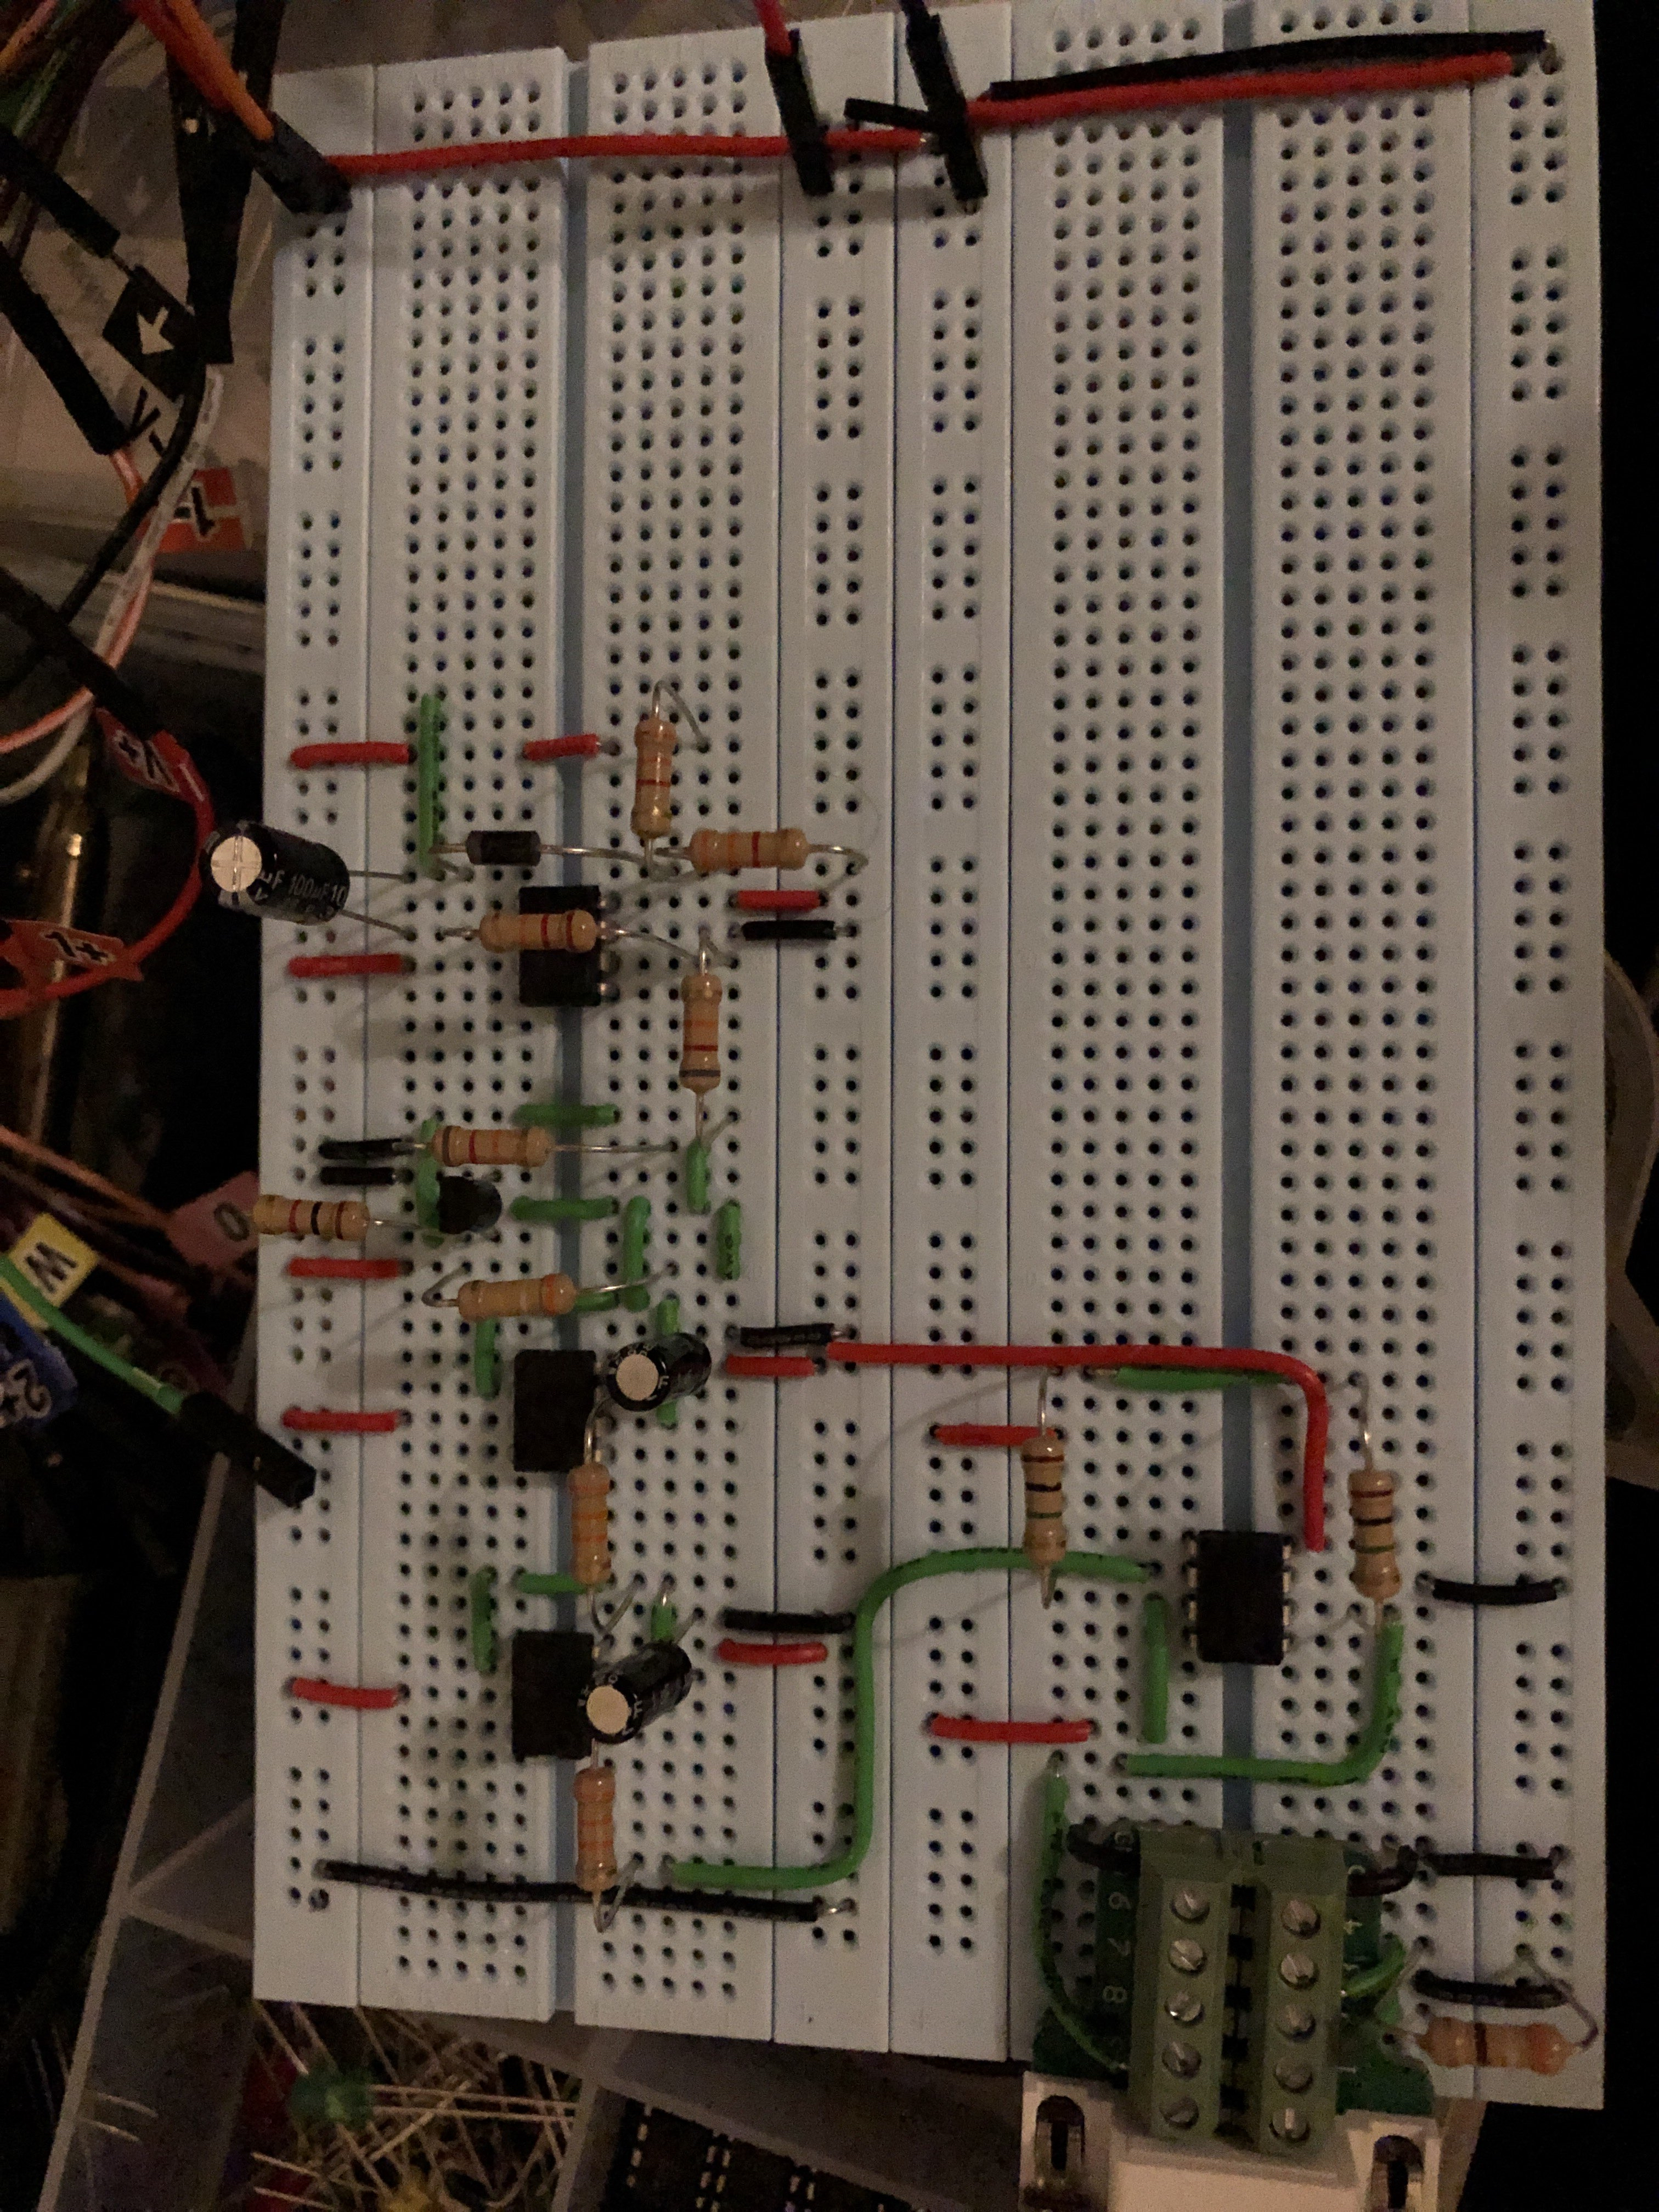
\includegraphics[width = .875\textwidth, height = .575\textwidth]{images/kavin_assembly_2.jpg}}
\end{center}
The next thing I did to assemble the circuit was to take the output of the previous sections, funnel it into the arduino and hooked the arduino up to the display
\begin{center}
    \boxed{\includegraphics[width = .875\textwidth, height = .575\textwidth]{images/kavin_complete_circuit.jpg}}
\end{center}
after that I rearranged some things and added in the multiplexer to choose between the two signals, red and ired. This will allow me to give the arduino enough information to calculate SPo2
\begin{center}
    \boxed{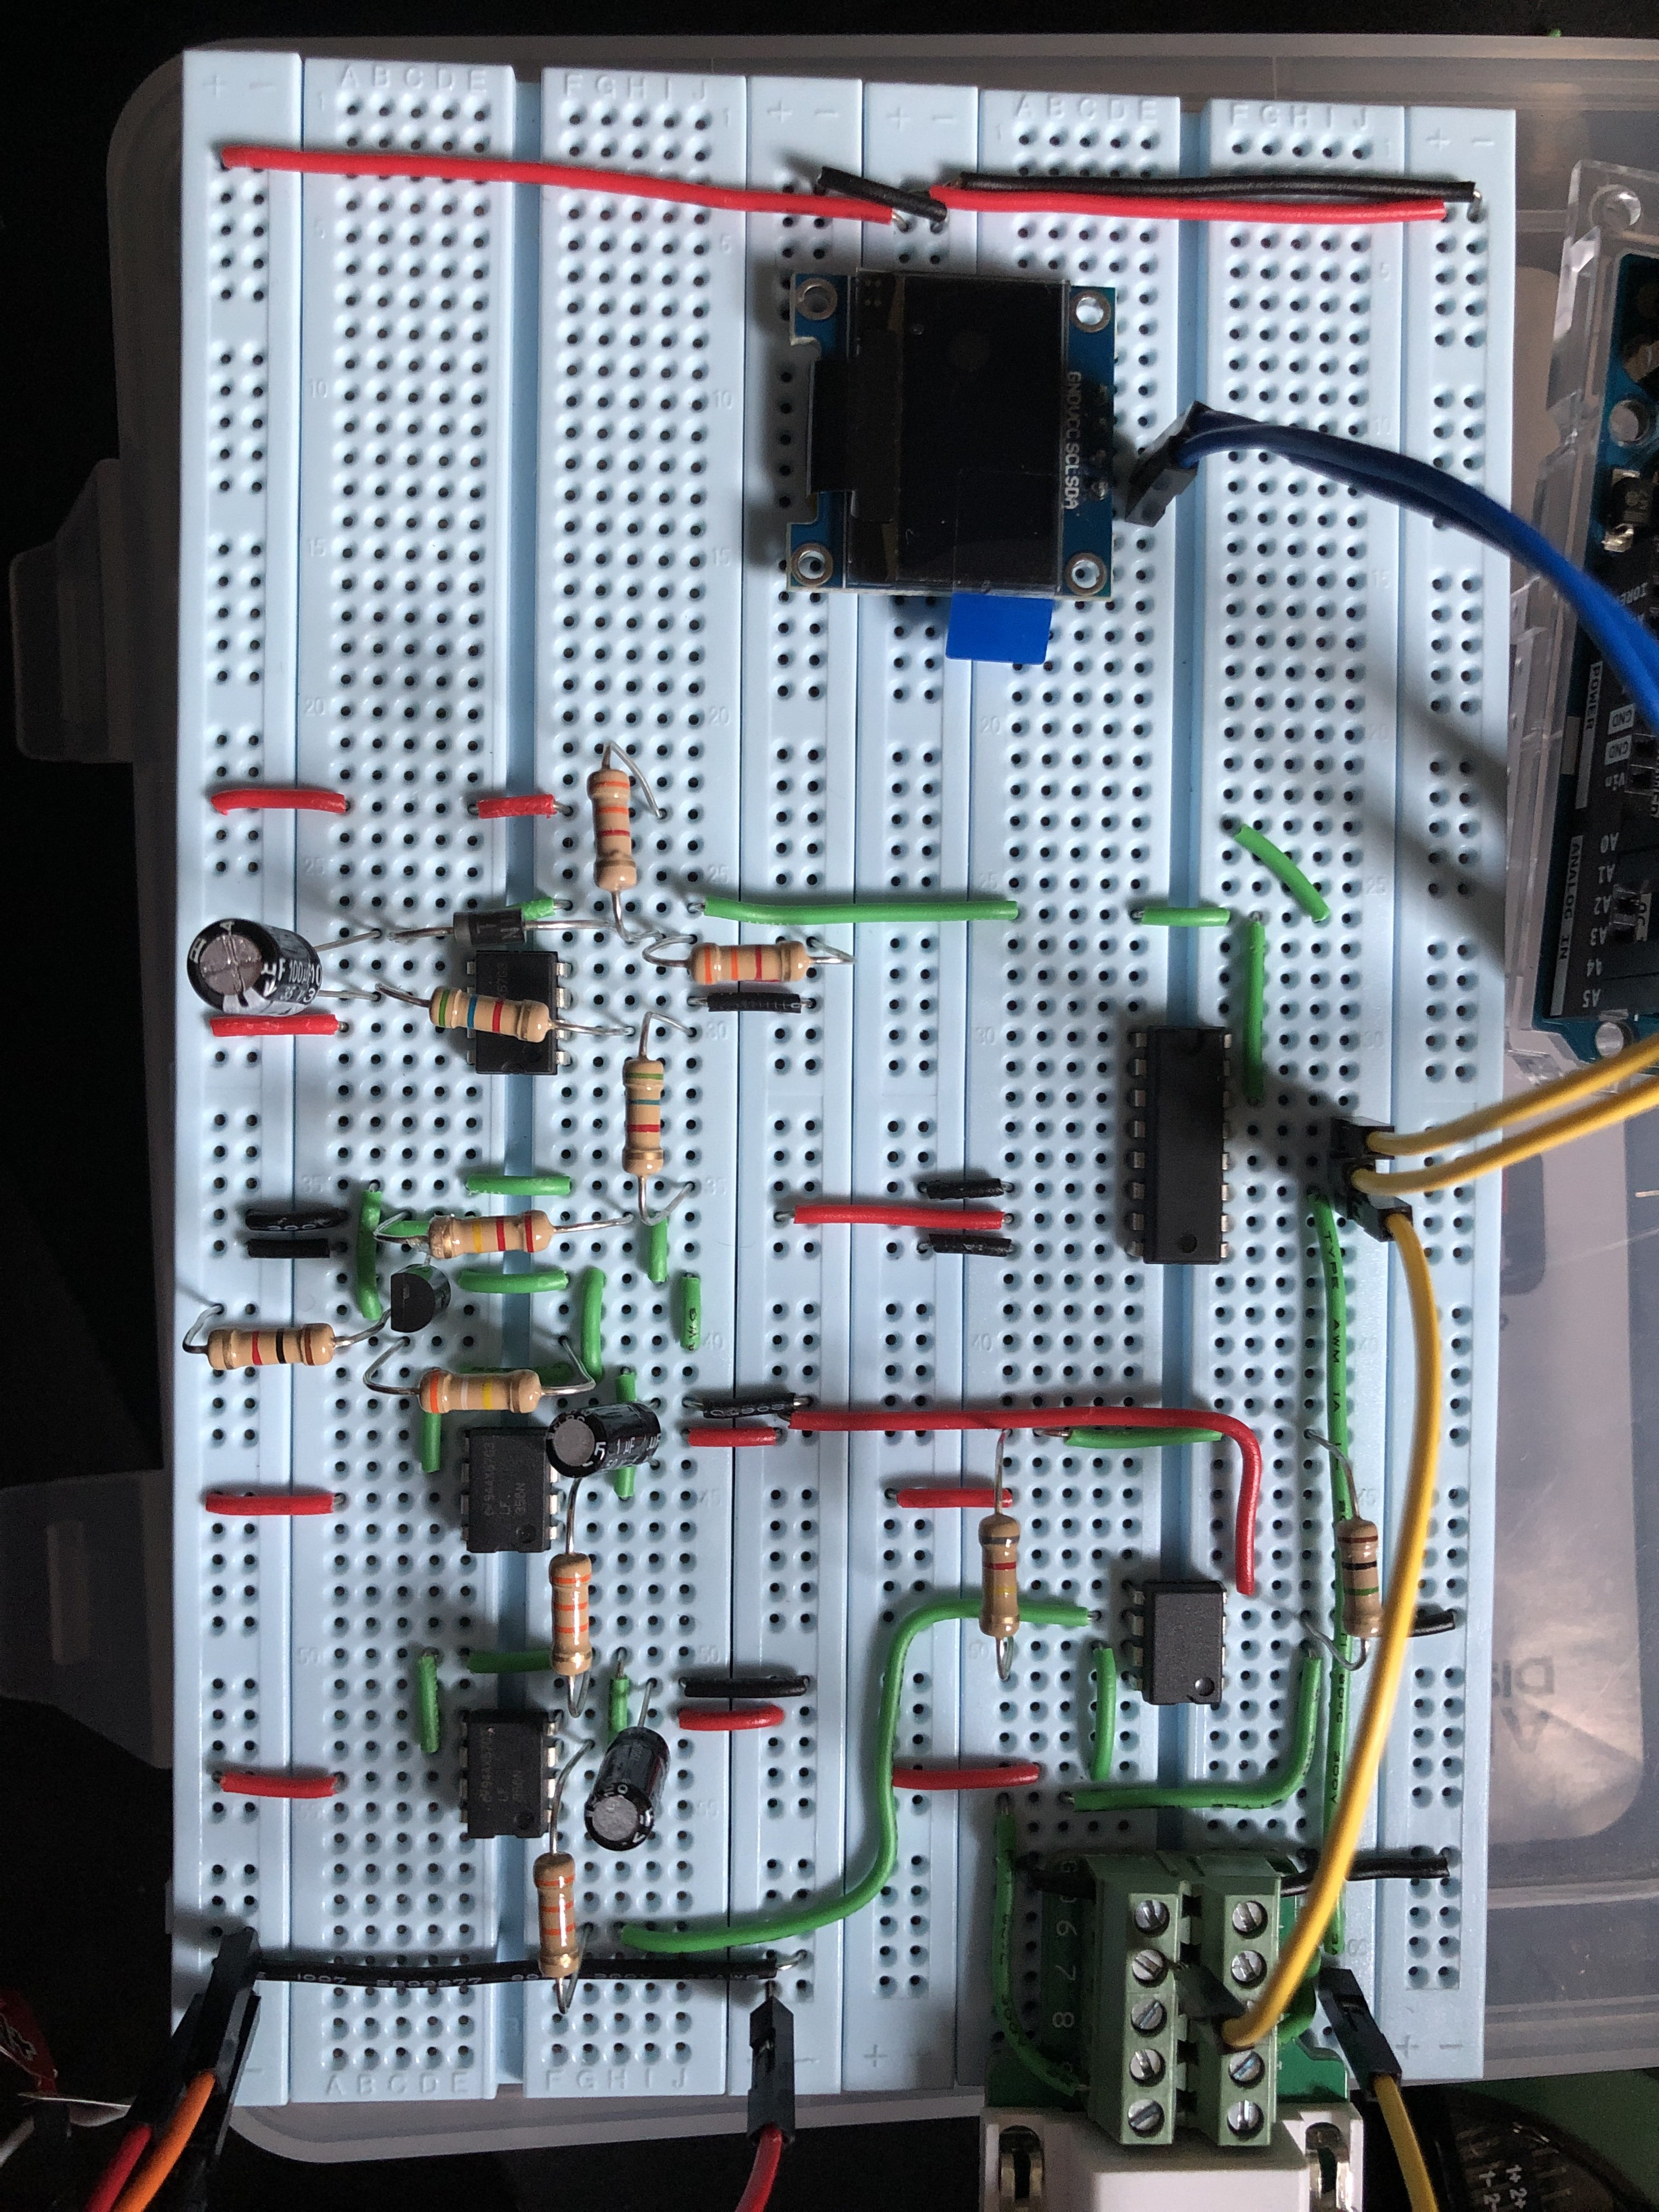
\includegraphics[width = .875\textwidth, height = .575\textwidth]{images/kavin_complete_circuit2.jpg}}
\end{center}
From here most of the circuitry is complete, some changes could be made in certain places to make the signal more consistent and easier to read, but since that is independent of rest of the programming and other changes, it can happen at any time.
\newpage
\section{Session 8 (Code Refactoring) [13 hours 46 minutes]}
here I redid most of my code, made it more organized and easy to read aswell as made SpO2 more consistent
\begin{lstlisting}[language=Arduino, caption= Complete  Code]
/**
  ECE2804 SpO2 Sensor Code
  Name: project_code
  Purpose: calculate heartrate and spo2 
            given cleaned signals from sensor

  @author Kavin Thirukonda
  @version 2.4 4/27/21
*/

//standard includes needed for display
#include <Wire.h> 
#include <SPI.h>
#include <Adafruit_GFX.h>
#include <Adafruit_SSD1306.h> 

//creating display object using screen size parameters
#define SCREEN_WIDTH 128 // OLED display width
#define SCREEN_HEIGHT 32 // OLED display height
Adafruit_SSD1306 display(SCREEN_WIDTH, SCREEN_HEIGHT, &Wire, -1);

//declaring graph printing variables
int circularBuffer[SCREEN_WIDTH]; 
int printptr = 0; 
int graphHeight = SCREEN_HEIGHT - 10;

//creating defines to use during programming to make code easier to read
#define SAMPLES_PER_PERIOD 60 
#define SAMPLES_STORED 10     
#define SMOOTHING 4           
#define BEAT_INDICATOR 12      
#define MEASURING_PERIOD 5
#define MAX_ADC_VALUE 1023

//preinitializing functions
void readRED();
void readIRED();
void calcR();
void calcHR();

//setting variables for pin locations
int sensorPin = A0; 
int REDLedPin = 3;
int IRLedPin = 4;
 
//variables needed for the bulk of calculations
float infaredIn[SMOOTHING], sumIR,lastIR, scanner, start;
float redIn[SMOOTHING], sumRED,lastRED;
int period, samples;
int samplesCounter = 0;
float infaredInSPO2[SAMPLES_PER_PERIOD],redInSPO2[SAMPLES_PER_PERIOD];
float maxInfared= 0;
float minInfared= 0;
float maxRed= 0;
float minRed= 0;
double R=0;
float oldR[SAMPLES_STORED];
int oldT[SAMPLES_STORED];
int spo2ptr = 0;
int heartrateptr = 0;
int readptr;
float avR = 0;
int avBPM=0;
int bpmprint;
int spo2print=0;
float beforeIR;
bool rising;
int riseDuration;
int n;
long int last_beat;

/**
  Setup function used to initialize certain variables to zero
  and set some settings.

  @param  none
  @return none
*/
void setup() {

   //Setting Baudrate of device
   Serial.begin(9600);

   //Ensuring buffer for  device is clear
   Serial.flush();

   //check if display is properly conectted, if not stop program
   if (!display.begin(SSD1306_SWITCHCAPVCC, 0x3C)) { 
     Serial.println(F("SSD1306 allocation failed"));
     for (;;); // Don't proceed, loop forever
   }

   //initalize display by clearing startup
   //setting font and text color 
   //as well as initial drawing position
   display.clearDisplay();
   display.setTextSize(1);
   display.setTextColor(WHITE, BLACK);
   display.setCursor(0, 0);
   display.display();
   delay(500);
   display.clearDisplay();

   //Setting various modes on pins using previously declared 
   //variables and arduino functions
   pinMode(sensorPin,INPUT);
   pinMode(REDLedPin,OUTPUT);
   pinMode(IRLedPin,OUTPUT);

   //Sets initial state of both LEDs to off
   digitalWrite(REDLedPin,LOW);
   digitalWrite(IRLedPin,LOW);

   //Intializes arrays to zero using memset function
   memset(infaredInSPO2, 0, SAMPLES_PER_PERIOD);
   memset(redInSPO2, 0, SAMPLES_PER_PERIOD);
   memset(oldT, 0, SAMPLES_STORED);
   memset(oldR, 0, SAMPLES_STORED);
   memset(infaredIn, 0, SMOOTHING);
   memset(redIn, 0, SMOOTHING);
   period=0; 
   samples=0;
   sumIR = 0; 
   sumRED=0; 
   readptr = 0; 
}

/**
  main program loop, contains all overarching logic for
  when certain numbers are calculated and the display logic.

  @param  none
  @return none
*/
void loop (){  
    //calls function to read RED LED, for more indepth explaination check appropriate funtion
    readRED();

    //calls function to read IRED LED, for more indepth explaination check appropriate funtion
    readIRED();

    //stores output from both previously called functions into an array which can be
    //processed to calculte SpO2
    infaredInSPO2[spo2ptr]=lastIR;
    redInSPO2[spo2ptr]=lastRED;

    //increments circular pointer used to fill the array which manages spo2 caluclations,
    //since the only information we need from this is the maximum and minimum values
    //order does not matter and placing them anywhere in the array works fine for us.
    spo2ptr++;
    spo2ptr %= SAMPLES_PER_PERIOD;

    //Increments counter to check how many "samples" have been taken, my definition of a 
    //sample is everytime the two readRED() and readIRED() functions are all called there
    //is new sample, it is the checked if the sample count is above a  threshold which will
    //be explained later, if it is then a new R value is caluclated.
    samplesCounter++;
    if(samplesCounter>=samples){
      //calls function to calculate R, for more indepth explaination check appropriate funtion
      calcR();  
    }

    //reset variables for average R value and average heartrate
    avR = 0;
    avBPM=0;
    //checks if the the last reading is above in magnitude to the reading just before the last reading,
    //if it is that implies that the funtion currently has a positive derivative, if the function is
    // rising continouously for 3(BEAT_INDICATOR) "sample" 20ms periods (MEASURING_PERIOD), and it was not
    //just at a beat the reading before, then we can be sure that  the current cycle contains a beat, so
    //we run the calculate HR function
    if (lastIR > beforeIR){
     riseDuration++;
     if (!rising && riseDuration > BEAT_INDICATOR) {
       //calls function to calculate HR, for more indepth explaination check appropriate funtion
        calcHR();
     }
   } else {
     //set conditions for wave if it has been determined that it is not trending upwards
     rising = false;
     riseDuration = 0;
   }
   //sets last reading to be stored as the reading before last for comparason with the next reading.
   beforeIR = lastIR;
   //uses general formula to caluclate spo2 value from R
   int SpO2 = -19 * avR + 112;
   //if the spo2 value is in a valid range i.e. has found enough valid readings, change the values 
   // of spo2print, and bpmprint to the new calculated values, which will then be printed on the next cycles
   if(avR != 0 && SpO2 <= 100 && SpO2 > 0){
      spo2print = SpO2;
      bpmprint = avBPM;
   }
   //checks if the value of spo2print is still its initial value of zero, and if it isnt then it prints
   //the calculated values to the screen if it is, then it prints a string to the screen which says
   // "Calculating..." to let the user know to keep their finger there.
   if(spo2print !=0){
      display.clearDisplay();
      display.setCursor(0, 0);
      int16_t  x1, y1;
      uint16_t w, h;
      display.getTextBounds("XX% SpO2 XXX bpm", 0, 0, &x1, &y1, &w, &h);
      display.setCursor(display.width() - w, 0);
      display.print(spo2print);
      display.print("% SpO2 ");
      display.print(bpmprint);
      display.print(" bpm");
   }else{
      display.clearDisplay();
      display.setCursor(0, 0);
      display.print("   Calibrating...");
   }
//Code used to print graph to screen, works by storing a series of inputs, 
//using a for loop to iterate through array and print it to the screen using 
//draw line helper which is detail below, it also uses a circular buffer 
//similar to other parts of the project
//   if(printptr >= display.width()){
//     printptr = 0;
//   }

//   int analogVal = analogRead(sensorPin);
//   circularBuffer[printptr++] = analogVal;
//   //for loops to draw the graph itself
//   int xPos = 0; 
//   for (int i = printptr; i < display.width(); i++){
//     int analogVal = circularBuffer[i];
//     drawLine(xPos, analogVal);
//     xPos++;
//   }
//   for(int i = 0; i < printptr; i++){
//     int analogVal = circularBuffer[i];
//     drawLine(xPos, analogVal);
//     xPos++;;
//   } 

   //displays new screen
   display.display();
   
   //increments read pointer, and if it is too high it gets rest using
   // the modulo functions circular increment property
   readptr++;
   readptr %= SMOOTHING;
}

/**
  Function used to turn on the IRED 
  signal and read datapoints from it

  @param  none
  @return none
*/
void readIRED(){
    //turn on infared LED and turn off RED LED
    digitalWrite(REDLedPin,LOW);
    digitalWrite(IRLedPin,HIGH);
    // set counter variable to zero
    n = 0;
    //record start time
    start = millis();
    //set sum value to zero
    scanner = 0.0;
    //take samples until you reach the end of the MEASURING_PERIOD
    do{
      scanner += analogRead (sensorPin);
      n++;
    }
    while (millis() < start + MEASURING_PERIOD);  
    //calculate average
    scanner /= n;  
    //record new value in various places it needs to be in
    sumIR -= infaredIn[readptr];
    sumIR += scanner;
    infaredIn[readptr] = scanner;
    lastIR = sumIR / SMOOTHING;  
}

/**
  Function used to turn on the RED 
  signal and read datapoints from it

  @param  none
  @return none
*/
void readRED(){
    //turn off infared LED and turn on RED LED
    digitalWrite(REDLedPin,HIGH);
    digitalWrite(IRLedPin,LOW);
    // set counter variable to zero
    n = 0;
    //record start time
    start = millis();
    //reset sum variable
    scanner = 0.0;
    //record values until you reach the end of the MEASURING_PERIOD
    do{
      scanner += analogRead (sensorPin);
      n++;
    }
    while (millis() < start + MEASURING_PERIOD);  
    //calculate average
    scanner /= n; 
    //record value in various place it needs to be in
    sumRED -= redIn[readptr];
    sumRED += scanner;
    redIn[readptr] = scanner;
    lastRED = sumRED / SMOOTHING;
}

/**
  Function used to calculate R ratio
  by finding maximum and minimum of 
  both signals and plugging the into a formula

  @param  none
  @return none
*/
void calcR(){
    //reset sample counter
    samplesCounter = 0;
    
    //having these values at the min and max 
    // makes sure that the values read from the 
    //array will replace the initial ones since they
    // must be larger or smaller than min or max
    maxInfared = 0; 
    minInfared=MAX_ADC_VALUE; 
    maxRed = 0; 
    minRed=MAX_ADC_VALUE;
    for(int i=0;i<SAMPLES_PER_PERIOD;i++) {
      if(infaredInSPO2[i]> maxInfared){
        maxInfared = infaredInSPO2[i];
      } 
      if(infaredInSPO2[i]>0 && infaredInSPO2[i]< minInfared ){
        minInfared = infaredInSPO2[i];
      }
      if(redInSPO2[i]> maxRed){
        maxRed = redInSPO2[i];
      }
      if(redInSPO2[i]>0 && redInSPO2[i]< minRed ){
        minRed = redInSPO2[i];
      }
      infaredInSPO2[i]=0;
      redInSPO2[i]=0;
    }
    R = ((maxRed-minRed)/minRed)/((maxInfared-minInfared)/minInfared);
}

/**
  Function used to calculate heartrate using an
  average of the last couple times between each
  heartbeat.

  @param  none
  @return none
*/
void calcHR(){
  rising = true;
  //adds current R value to average array
  oldR[heartrateptr] = R;
  //adds current period length to average array
  oldT[heartrateptr] = millis() - last_beat;
  //stores time of last beat for next cycle
  last_beat = millis();
  //averages the R value aswell as the period
  int period = 0;
  for(int i =0; i<SAMPLES_STORED; i++){
    period += oldT[i];
  }
  period /= SAMPLES_STORED;
  samples = period / (2*MEASURING_PERIOD);
  int avPeriod = 0;
  for(int i =1; i<SAMPLES_STORED; i++) {
        avPeriod += oldT[i];
        avR += oldR[i];
  }  
  //modifys the pointer which controls the heartrate array
  heartrateptr++;
  heartrateptr %= SAMPLES_STORED;
  //calculates average R  and T from average R sum and T sum
  avR = avR / SAMPLES_STORED ;
  avPeriod /= SAMPLES_STORED;
  //calculates heart rate by dividing 60 seconds by the average period
  avBPM = 60000 / avPeriod;
}

/**
  Function to draw vertical line
  given an x-position and analog
  value, for drawing graph.

  @param  xPos to print on
  @param  analogValue to print up to  
  @return none
*/
void drawLine(int xPos, int analogVal){
  int lineHeight = map(analogVal, 0, MAX_ADC_VALUE, 0, graphHeight);
  int yPos = display.height() - lineHeight;
  display.drawFastVLine(xPos, yPos, lineHeight, SSD1306_WHITE);
}
\end{lstlisting}
\newpage
\section{Session 9 (Finalization) [2 hours 34 minutes]}
I have the final iteration of the circuit built now
\begin{center}
    \boxed{\includegraphics[width = \textwidth, height = .6\textwidth]{images/image0.jpg}}
\end{center}
The end goal of the project is completely achieved, both SpO2 and heartrate are being calculated, if there is one thing I wish I could have done better would be to make the graph display be more consistent than it currently is, right now its very fidgety and only works sometimes, but overall im happy with the result of the project.
\section{Sources}
\begin{itemize}
    \item \url{https://www.ti.com/general/docs/suppproductinfo.tsp?distId=10&gotoUrl=http%3A%2F%2Fwww.ti.com%2Flit%2Fgpn%2Fcd4051b}
    \item \url{https://www.edn.com/signal-processing-and-calibration-improve-blood-measurements/}
    \item \url{https://www.ti.com/lit/ds/symlink/lf356.pdf?ts=1617382462054&ref_url=https%253A%252F%252Fwww.ti.com%252Fproduct%252FLF356}
    \item \url{https://www.ncbi.nlm.nih.gov/pmc/articles/PMC6651860/#:~:text=Heart%20rate%20is%20calculated%20by,device%20in%20the%20dry%20environment.}
    \item \url{https://www.ncbi.nlm.nih.gov/pmc/articles/PMC6595535/#C14}
\end{itemize}
\end{document}
